% per commentare una riga mettere % al suo inizio
% per s-commentare una riga (ossia attivarla) togliere il % al suo inizio
%
\documentclass[pdfa% formato PDF/A, obbligatorio per l'archiviazione delle tesi di Polito
,cucitura%lascia margine per la rilegatura
%,twoside% per stampa fronte-retro (fortemente consigliato per tesi voluminose, opzionale per le altre)
%,12pt% font pi� grande (12pt) rispetto a quello normalmente usato (11pt)
]{toptesi}
%
% Commentare le righe seguenti se NON si � specificata l'opzione "pdfa"
\hypersetup{%
    pdfpagemode={UseOutlines},
    bookmarksopen,
    pdfstartview={FitH},
    colorlinks,
    linkcolor={black},
    citecolor={red},
    urlcolor={blue}
  }
% \documentclass[11pt,twoside,oldstyle,autoretitolo,classica,greek]{toptesi}
% \usepackage[or]{teubner}
%%%%%%%%%%%%%%%%%%%%%%%%%%%%%%%%%%%%%%%%%%%%%%%%%%%%
%
% Esempio di composizione di tesi di laurea.
%
% Questo esempio e' stato preparato inizialmente 13-marzo-1989
% e poi e' stato modificato via via che TOPtesi andava
% arricchendosi di altre possibilita'.
%
% Nel seguito laurea "quinquennale" sta anche per "specialistica" o "magistrale"

% Cambiare encoding a piacere; oppure non caricare nessun encoding se si usano
% solo caratteri a 7 bit (ASCII) nei file d'entrata.
%
\usepackage[latin1]{inputenc}% IMPORTANTE! usare codifica ISO-8859-1 per le lettere accentate


%
%\chapterbib %solo per vedere che cosa succede; e' preferibile comporre una sola bibliografia
%\AdvisorName{Supervisors}
%\newtheorem{osservazione}{Osservazione}% Standard LaTeX

%\usepackage[a-1b]{pdfx}
%\hypersetup{%
%    pdfpagemode={UseOutlines},
%    bookmarksopen,
%    pdfstartview={FitH},
%    colorlinks,
%    linkcolor={blue},
%    citecolor={green},
%    urlcolor={blue}
%  }

%
% per numerare e far comparire nell'indice anche le sezioni di quarto livello
% SCONSIGLIATO! da usarsi solo in caso di estrema necessit�
\setcounter{secnumdepth}{4}% section-numbering-depth
\setcounter{tocdepth}{4}% TOC-numbering-depth (TOC=Table-Of-Content)

%\setbindingcorrection{3mm}

% Set default language (if not defined, then is "italiano"
% To switch to other language during writing, use \selectlanguage{language}
\english


%%%%%%%%%%%%%%%%%%%%%%%%%%%%%%%%%%%%%%%%%
%%%%%%% Change the strings if you want a title page and a copyright page
%%%%%%% in another language
%%%%%%% Comment just the \iflanguage statement and the closing line of the language test
%%%%%%% if you want to make a global change instead of a conditional one.
%%%%%%% Comment the following indented lines if you don't care about the title page
%%%%%%% in English
\iflanguage{english}{%
	%\retrofrontespizio{This work is subject to the Creative Commons Licence}
	\DottoratoIn{PhD Course in\space}
	\CorsoDiLaureaIn{Master in\space}
	\NomeMonografia{Bachelor Degree Final Work}
	\TesiDiLaurea{Master Thesis}
	\NomeDissertazione{PhD Dissertation}
	\InName{in}
	\CandidateName{Candidates}% or Candidate
	\AdvisorName{Supervisors}% or Supervisor
	\TutorName{Tutor}
	\NomeTutoreAziendale{Internship Tutor}
	\CycleName{cycle}
	\NomePrimoTomo{First volume}
	\NomeSecondoTomo{Second Volume}
	\NomeTerzoTomo{Third Volume}
	\NomeQuartoTomo{Fourth Volume}
}{}
%%%%%%%%%%%%%%%%%%%%%%%%%%%%%%%%%%%%%%%%%



\ateneo{Politecnico di Torino}

%%% scegliere la propria facoltà (solo PRIMA dell'AA 2012-2013)
%
%\facolta[III]{Ingegneria dell'Informazione}
%\facolta[IV]{Organizzazione d'Impresa\\e Ingegneria Gestionale}
%\Materia{Remote sensing}% uso sconsigliato
\FacoltaDi		% no facoltà di voice
\facolta			% no facoltà name

%\monografia{Gestione informatizzata di un magazzino ricambi}% per la laurea triennale
\titolo{Oculus Rift and AR}% per la laurea quinquennale e il dottorato
%\sottotitolo{Metodo dei satelliti medicei}% NON obbligatorio, per la laurea quinquennale e il dottorato

%%% scegliere il proprio corso
%
%\corsodilaurea{Ingegneria dell'Organizzazione d'Impresa}% per la laurea di primo e secondo livello
%\corsodilaurea{Ingegneria Logistica e della Produzione}% per la laurea di primo e secondo livello
%\corsodilaurea{Ingegneria Gestionale}% per la laurea di primo e secondo livello
\corsodilaurea{Computer Engineering}% per la laurea di primo e secondo livello
%\corsodidottorato{Meccanica}% per il dottorato

\candidato{Giovanni \textsc{Pautasso}}% per tutti i percorsi
%\secondocandidato{Evangelista \textsc{Torricelli}}% per la laurea magistrale solamente
%\direttore{prof. Albert Einstein}% per il dottorato
%\coordinatore{prof. Albert Einstein}% per il dottorato
\relatore{prof.\ Antonio Lioy}% per la laurea e il dottorato
%\secondorelatore{dipl.~ing.~Werner von Braun}% per la laurea magistrale
%\terzorelatore{{\tabular{@{}l}dott.\ Neil Armstrong\\prof. Maria Rossi\endtabular}}% per la laurea magistrale
%\tutore{ing.~Karl Von Braun}% per il dottorato
%\tutoreaziendale{dott.\ ing.\ Giovanni Giacosa} % solo per la laurea di secondo livello con tesi svolta in azienda
%\NomeTutoreAziendale{Supervisore aziendale\\Centro Ricerche FIAT}
%\sedutadilaurea{Agosto 1615}% per la laurea quinquennale
%\esamedidottorato{Novembre 1610}% per il dottorato
\sedutadilaurea{\textsc{Dicembre} 2015}% per la laurea triennale
%\sedutadilaurea{\textsc{Anno~accademico} 1615-1616}% per la laurea magistrale
%\annoaccademico{1615-1616}% solo con l'opzione classica
%\annoaccademico{2006-2007}% idem
%\ciclodidottorato{XV}% per il dottorato
\logosede{sections/frontespizio/logopolito}

% per inserire uno spazio "fantasma" nella definizione di un'abbreviazione
\usepackage{xspace}

% per inserire un DOI senza problemi coi caratteri "strani" ivi presenti
\usepackage{doi}
\renewcommand{\doitext}{DOI }% originally was "doi:"

% per inserire correttamente le unit� di misura SI (incluse quelle binarie)
\usepackage[binary-units]{siunitx}
% se si desidera usare / invece che la potenza -1 per indicare "al secondo"
\sisetup{per-mode=symbol}

% per inserire codice di programmazione complesso
\usepackage{listings}% per inserire codice di programmazione complesso
\lstset{
basicstyle=\ttfamily,
columns=fullflexible,
xleftmargin=3ex,
breaklines,
breakatwhitespace,
escapechar=`
}

% modify some page parameters
\setlength{\parskip}{\medskipamount}
\advance\voffset -5mm
\advance\textheight 30mm

% riga orizzontale
\newcommand{\HRule}{\rule{\linewidth}{0.2mm}}
% esempio di creazione di semplici abbreviazioni
\newcommand{\ltx}{\LaTeX\xspace}
\newcommand{\txw}{TeXworks\xspace}
\newcommand{\mik}{MikTex\xspace}
\newcommand{\html}{HTML\xspace}
\newcommand{\xhtml}{XHTML\xspace}

% esempio di creazione di un'abbreviazione con un parametro (il cui uso � indicato da #1)
\newcommand{\cmd}[1]{\texttt{#1}\xspace}
% per citare un RFC, es. \rfc{822}
\newcommand{\rfc}[1]{RFC-#1\xspace}
% per citare un file (es. \file{autoexec.bat}) o una URI fittizia (es. \file{http://www.lioy.it/})
% per le URI vere usare \url o \href
\newcommand{\file}[1]{\texttt{#1}\xspace}
% per inserire codice di esempio in-line
\newcommand{\code}[1]{\lstinline|#1|}
% importante per i pathname Windows perch� non si pu� usare \ essendo un carattere riservato di Latex
\newcommand{\bs}{\textbackslash}
% definizione di un termine: formattazione ed inserimento nell'indice
\newcommand{\tdef}[1]{\textit{#1}\index{#1}}
% meta-termine, usato tipicamente nelle definizioni dei tag
\newcommand{\meta}[1]{\textit{#1}}

% better aligment for overbrace command
\newcommand{\xoverbrace}[2][\vphantom{\dfrac{A}{A}}]{\overbrace{#1#2}}
\newcommand{\pder}[2]{\frac{\partial#1}{\partial#2}}

\begin{document}



\errorcontextlines=9

\expandafter\ifx\csname StileTrieste\endcsname\relax
    \frontespizio
\else
    \paginavuota
    \begin{dedica}
        A mio padre

        \textdagger\ A mio nonno Pino
    \end{dedica}
    \tomo
\fi

% COMMENT OUT TO REMOVE THE FOLLOWING SECTIONS

% prints summary of the content
\sommario

Inserire qui un breve sommario della tesi.

% prints acknowledgements and special thanks
\ringraziamenti

Opzionali, solo nel caso si sia ricevuto un aiuto speciale e particolarmente rilevante.

%% inserire sempre nella tesi per la laurea di I livello, perché il nome dei tutori non è indicato sul frontespizio.
%Il lavoro descritto in questa monografia è stato svolto sotto la supervisione
%del Prof. Antonio Lioy (tutore accademico)% inserire sempre il nome del tutore accademico
% e dell'Ing. Mario Rossi (tutore aziendale)% inserire solo se la monografia è relativa ad un tirocinio.
%.



%\tablespagetrue % normalmente questa riga non serve ed e' commentata
%\figurespagetrue % normalmente questa riga non serve ed e' commentata

% prints the thesis index section
\indici

% start chapter enumeration
\mainmatter

\chapter{Introduction}
%\section{Scrittura di un capitolo}

Dividere la tesi in capitoli (col comando \cmd{\bs chapter}) ed il capitolo in parti logiche mediante gli appositi comandi (\cmd{\bs section}, \cmd{\bs subsection} e \cmd{\bs subsubsection}).

Cercare inoltre di scrivere in  buon italiano perch� la tesi � un documento formale che viene archiviato per lungo tempo e costituisce parte della carriera di uno studente.

Questo capitolo di esempio contiene informazioni circa l'uso del sistema \ltx per la scrittura di testi scientifici (molto utile anche per la composizione della tesi di laurea).
Si consiglia di non limitarsi solo a leggere questo testo ma di esaminare il file \file{.tex}  corrispondente per imparare rapidamente i comandi \ltx tramite gli esempi contenuti in tale file sorgente.

\section{Installazione di un sistema \ltx}

Esistono tanti sistemi per elaborare testi scritti in \ltx. Per sistemi Windows si consiglia l'uso di \mik, che pu� essere scaricato dal seguente sito:

\url{http://www.miktex.org/}

\mik installa automaticamente anche \txw, un IDE (Integrated Development Environment) per \ltx che permette di scrivere il sorgente ed ottenere velocemente il PDF corrispondente, che viene mostrato in una finestra separata. \txw � integrato con un correttore ortografico ed � dotato di auto-completamento delle parole (ad esempio scrivendo \cmd{bit} e premendo quindi TAB viene generato automaticamente l'ambiente \cmd{itemize} per inserire una lista non ordinata); si veda la sezione 6.3 del \href{http://www.leliseron.org/texworks/}{manuale} di \txw per un elenco completo.
Notare anche che facendo click col tasto destro nella finestra che visualizza il PDF � possibile saltare automaticamente al punto corrispondente nella finestra di edit e viceversa.

%%%%%%%%%%

\section{Comporre testi con \ltx}

In questa sezione vengono fornite alcune informazioni generali sull'uso del linguaggio \ltx per comporre testi complessi.

%%%%%%%%%%

\subsection{Testo normale}

Le lettere accentate\index{accenti} si possono scrivere direttamente (mediante i tasti presenti sulla propria tastiera) se si � specificata la codifica ISO-8859-1 in \mik:
\begin{verbatim}
  Edit > Preferences > Editor > Encoding > ISO-8859-1
\end{verbatim}
Altrimenti si possono usare le sequenze di escape (attenzione a quella per la lettera i accentata):
\`a, \`e, \'e, \`{\i}, \`o, \`u.

Si ricordi che in Italiano l'accento � quasi sempre grave. L'accento acuto si usa in pochi casi specifici, quali le parole perch�, poich� e finch�, o la coppia n� \ldots n�.

I segni di interpunzione devono essere attaccati alla parola che li precede e separati con uno spazio dalla parola che li segue:
\begin{quote}
(giusto) ``caspita, che bella notizia!''
\\
(sbagliato) ``caspita , che bella notizia!''
\\
(sbagliato) ``caspita ,che bella notizia!''
\end{quote}

L'apostrofo\index{apostrofo} deve essere attaccato sia alla parola che lo procede sia a quella che lo segue:
\begin{quote}
(giusto) ``l'oro � un metallo prezioso''
\\
(sbagliato) ``l' oro � un metallo prezioso''
\\
(sbagliato) ``l 'oro � un metallo prezioso''
\\
(sbagliato) ``l ' oro � un metallo prezioso''
\end{quote}

Lasciando una riga vuota si genera automaticamente un nuovo paragrafo,\index{paragrafo} ossia si va a capo, si lascia un piccolo spazio verticale e si indenta la prima riga del paragrafo.
E' importante cercare di organizzare il proprio testo in paragrafi che contengano insieme di frasi correlate. Quando si cambia argomento, si inizia un nuovo paragrafo. Si puo considerare questo testo come un buon esempio di suddivisione in paragrafi.

L'uso del comando \cmd{\bs\bs} per forzare un ritorno a capo � fortemente deprecato. In sua vece bisogna usare il comando corrispondente all'effetto che si desidera ottenere: ad esempio, se � terminato un paragrafo basta lasciare una riga vuota, se si vuole creare un elenco basta usare uno dei comandi per la creazione di una lista.

Attenzione ai doppi apici \index{virgolette} che devono essere creati usando due volte il tipo di apice appropriato (aperto o chiuso), come nel seguente caso:
\begin{quote}
il film ``Il Ciclone'' � stato diretto ed interpretato da Leonardo Pieraccioni.
\end{quote}
Se alcune parole ricorrono frequentemente nel testo e sono scritte in un modo particolare allora conviene definire un'opportuna abbreviazione nel preambolo del file, ossia prima di \cmd{\bs begin\{document\}}. Come esempi si vedano in questo file le definizioni e l'uso delle abbreviazioni \cmd{\bs ltx} per generare la parola \ltx e \cmd{\bs cmd} per presentare in modo opportuno i comandi.

E' anche facile creare delle note\index{note} a pi� di pagina\footnote{\ldots ma vanno usate con parsimonia.} che vengono numerate automaticamente.

Non bisogna dimenticare di usare un correttore ortografico. Per installare il dizionario necessario scaricare dal sito \url{http://wiki.services.openoffice.org/wiki/Dictionaries} il file ZIP corrispondente alla lingua prescelta (nel caso sia la lingua Inglese installare il dizionario British e non American) e quindi estrarre tutti i file nella  cartella
\begin{center}
\cmd{C:\bs Program Files\bs MiKTeX 2.9\bs hunspell\bs dicts}
\end{center}
Il correttore si attiva quindi scegliendo il men�:
\begin{verbatim}
  Edit > Spelling > lingua_desiderata
\end{verbatim}
Le parole errate compariranno evidenziate con una sottolineatura in rosso: sar� cos� possibile modificarle direttamente oppure -- cliccandoci sopra col tasto destro -- scegliere tra le opzioni di correzione proposte.

E' possibile scrivere parti della tesi in lingue diverse, specificando il linguaggio usato (importante in modo che il programma vada a capo in modo corretto). Segue una citazione in inglese:
\selectlanguage{english}
\begin{quotation}
The man in the rubber boots and a thick coat to protect against the evening chill walked purposefully about a farm here, scattering pheasants as he went. He could have been an English gentleman out for a bit of hunting, except he carried no gun.

In his current circumstance, the WikiLeaks founder Julian Assange is more hunted than hunter, fighting extradition to Sweden on accusations of sexual misconduct while struggling to maintain the influence of WikiLeaks even as he remains here at Ellingham Hall, the country manor house of Vaughan Smith, a former soldier and journalist who runs a restaurant and club for journalists in London. 
\end{quotation}
\selectlanguage{italian}
Adesso si riprende il normale testo in Italiano, che seguir� le regole di composizione della lingua Italiana.

\index{citazioni!testuali}
Per inserire citazioni testuali (ossia porzioni di testo) si pu� usare l'ambiente \cmd{quote} (citazione breve) oppure quello \cmd{quotation} (per citazioni lunghe, che posso essere composte da pi� paragrafi), come appena fatto qui sopra per la citazione in inglese.

\index{URL}
Per inserire collegamenti a pagine o documenti web si usano i comandi \cmd{\bs url} e \cmd{\bs href} del package \file{hyperref} come nei due seguenti esempi:
\begin{description}
\item[uso di \cmd{\bs href}]\mbox{}\\
(sorgente) \verb+Nel \href{http://www.polito.it/}{sito web} del Politecnico di Torino+
\\
(risultato) Nel \href{http://www.polito.it/}{sito web} del Politecnico di Torino
\item[uso di \cmd{\bs url}]\mbox{}\\
(sorgente) \verb+Il sito web del Politecnico di Torino � \url{http://www.polito.it/}+
\\
(risultato) Il sito web del Politecnico di Torino � \url{http://www.polito.it/}
\end{description}

\index{citazioni!bibliografiche}
Infine � possibile citare testi o siti che sono stati consultati per la tesi: articoli a congresso \cite{psisec},
articoli su rivista \cite{tpa}, capitoli di libri \cite{tc}, siti o pagine web \cite{openssl} e RFC (come \rfc{5246} \cite{tls12} che definisce la versione 1.2 del protocollo TLS).
Si noti che le voci della bibliografia devono essere elencate nell'apposita sezione (comando \cmd{\bs thebibliography}) secondo l'ordine in cui vengono citate.
Per bibliografie pi� complesse � possibile l'uso di BibTex, ma � sconsigliato se non si supera la decina di citazioni.

%%%%%%%%%%

\subsection{Liste}

\index{liste!non ordinate}
Usare liste puntate per elenchi in cui l'ordine non � importante, come nel caso degli esami obbligatori da superare per essere ammessi al secondo anno:
\begin{itemize}
\item
Analisi Matematica I;
\item
Fisica I;
\item
un esame a scelta tra Chimica ed Informatica.
\end{itemize}
Notare che normalmente ogni elemento della lista � costituito da un'unica frase, terminata da punto-e-virgola, tranne l'ultimo elemento che � terminato da un punto. Ogni punto inizia con lettera minuscola (a meno che la parola iniziale sia un sigla o un nome proprio). E' fortemente sconsigliato l'uso di una lista se uno o pi� punti contengono pi� di una singola frase. In questo caso conviene scrivere paragrafi separati oppure creare delle sottosezioni.

\index{liste!ordinate}
Le liste numerate si creano con l'ambiente \cmd{enumerate} e sono utili per elencare elementi aventi un ordine di priorit�, come nel caso della ricetta per cucinare la pastasciutta:
\begin{enumerate}
\item
prendere una pentola;
\item
riempirla di acqua;
\item
metterla sul fuoco e portare l'acqua ad ebollizione;
\item
quando l'acqua bolle, buttare la pasta;
\item
quando la pasta � cotta, scolarla, condirla e \ldots mangiarla!
\end{enumerate}
\index{liste!di descrizioni}
Si possono anche fare delle liste che servono per descrivere generici oggetti, usando l'ambiente \cmd{description}.
L'oggetto descritto viene automaticamente posizionato ad inizio riga e scritto in grassetto, come nel seguente esempio:
\begin{description}
\item[pentola]
oggetto metallico usato per cuocere cibi;
\item[mela]
frutto che fa molto bene alla salute;
\item[Sarchiapone] animale immaginario usato in una gag di Walter Chiari e poi ripreso in un programma radiofonico da Renzo Arbore.
\end{description}

%%%%%%%%%%

\subsection{Formule matematiche ed unit� di misura}

\index{formule matematiche}
Le formule matematiche si possono scrivere direttamente nel corpo del testo racchiudendole tra due simboli \verb+$+
(come in questo esempio per il calcolo della circonferenza, $c = 2 \pi r$)
oppure scrivere la formula su una riga centrata racchiudendola tra \verb+\[+ e \verb+\]+:
\[
c = 2 \pi r
\]
Apici, pedici, frazioni, puntini e sommatorie sono anche semplici da fare:
\[
k = a_0 + a_1 \frac{1}{x} + a_2 \frac{1}{x^2} + \dots = \sum_{i=0}^N a_i \frac{1}{x^i} = \sum_{i=0}^N a_i x^{-i}
\]
Ecco ora un esempio di limite:
\[
\lim_{x\to\infty}f(x)=0
\]
\index{unit� di misura}
Quando si usano delle grandezze fare attenzione alle unit� di misura: usare sempre il SI e scrivere correttamente i simboli (ad esempio, il simbolo del chilo � la lettera ``k'' minuscola non la ``K'' maiuscola).
Per evitare errori e lasciare il giusto spazio tra quantit� e simbolo si suggerisce l'uso del package \cmd{siunitx} che aggiunge i comandi \cmd{\bs si} per unit� isolate o \cmd{\bs SI} per quantit� numerica seguita dalla sua unit� di misura.
Ecco un esempio d'uso per citare unit� isolate:
\begin{quote}
\ldots fornire il risultato in \si{\square\centi\metre}.
\end{quote}
ma � anche possibile indicare l'unit� su quantit� numeriche specifiche, citate in-line (ad esempio, un sacco di patate da \SI{10}{\kilo\gram}) o all'interno di una formula matematica:
\[
v = \frac{s}{t} = \frac{ \SI{100}{\meter} }{ \SI{5}{\second} } = \SI{20}{\meter\per\second}
\]

Nel caso di unit� relative al sistema binario � possibile adottare sia la vecchia notazione, che usa gli stessi prefissi del SI ma sottointende l'uso delle potenze di 2, sia la nuova notazione, in cui i prefissi del sistema binario sotto caratterizzati da una ``i'' minuscola.
Ad esempio:
\[
\SI{1}{\tera\byte}\ \mbox{(vecchia notazione)} =
\SI{1}{\tebi\byte}\ \mbox{(nuova notazione)} =
2^{30} \si{\byte}
\]

%%%%%%%%%%

\subsection{Tabelle e figure}

\index{tabelle}
In \ltx le tabelle si compongono descrivendo le righe di cui sono composte:
\begin{center}
\begin{tabular}{|l|c|c|}% posizionamento del testo nelle colonne l:left c:center r:right
\hline
\textit{modello} & \textit{velocit�} & \textit{consumi} \\
                 & [ \si{km/h} ]          & [ l/\SI{100}{km} ] \\
\hline
Fiat 500 & 150 & 19 \\
Alfa Giulietta & 210 & 21.5 \\
Ferrari Testarossa & 320 & 5.7 \\
\hline
\end{tabular}
\end{center}
Normalmente � meglio non inserire le tabelle direttamente nel testo ma creare un oggetto separato, con una didascalia ed un numero per citarlo ove necessario. Ad esempio � stata creata in questo modo la tabella~\ref{tab:voti} che riporta i voti conseguiti in alcuni esami da un ipotetico studente ma � slegata da questo specifico paragrafo. In questo modo \ltx sistemer� la tabella in un punto opportuno del testo, evitando di lasciare spazio verticale inutilizzato.
Si noti l'uso del carattere ``tilde'' (\textasciitilde) per tenere legato il numero della tabella (o figura o altro elemento flottante) alla parola che lo precede.

\begin{table}[tbh] % per piazzare la tabella t:top b:bottom h:here in ordine di preferenza; h � sconsigliato
\begin{center}
\begin{tabular}{|l|c|c|}
\hline
\textit{esame} & \textit{data} & \textit{voto} \\
\hline
Analisi I & 27/1/2009 & 18 \\
Informatica & 14/2/2009 & 30 \\
Fisica I & 15/7/2009 & 27 \\
\hline
\end{tabular}
% \caption contiene il testo della didascalia: limitarsi ad un una sola riga
% notare l'uso di \label per creare un'etichetta per citare la figura tramite \ref
% N.B. quando ci sono label o indici bisogna sempre elaborare due volte il file latex perch� la prima crea i riferimenti e la seconda li inserisce
\caption{Voti riportati negli esami sinora sostenuti.\label{tab:voti}}
\end{center}
\end{table}

\index{figure}
Per quanto riguarda le figure, conviene disegnarle con un apposito programma (es. PowerPoint) e poi salvarle in un file che verr� richiamato nel file \ltx. Si consiglia di prestare attenzione ai font usati (suggeriti Arial o Helvetica), alla dimensione (minimo \SI{10}{pt}) e di generare un formato grafico ad alta definizione (PDF � il preferito, altrimenti PNG o JPG ad alta qualit�).
Il file grafico verr� poi incluso in \ltx per generare la figura, come nell'esempio della figura~\ref{fig:popTorino} che riporta il grafico della variazione di popolazione della citt� di Torino.
Si noti che questo grafico � di bassa qualit� (pixel percepibili ad occhio nudo) perch� salvato come JPG a bassa risoluzione (solo \SI{96}{DPI}).
Per i formati raster si dovrebbe sempre usare una risoluzione di almeno \SI{300}{DPI}.
%
\begin{figure}[tbh]% per piazzare la tabella t:top b:bottom h:here, in ordine di preferenza; h � sconsigliato
\centerline{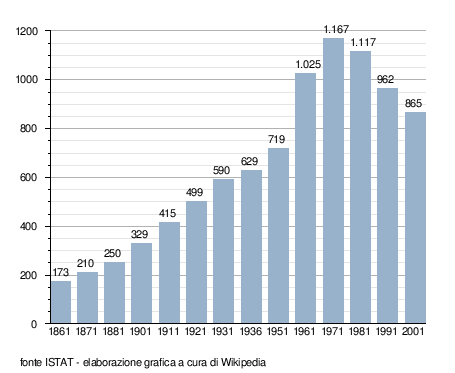
\includegraphics[width=0.9\textwidth]{torino.png}}
\caption{Popolazione di Torino, in migliaia di abitanti (fonte: \href{http://it.wikipedia.org/wiki/Torino}{wikipedia}).\label{fig:popTorino}}
\end{figure}
%
Nel caso che la figura non abbia gi� la dimensione desiderata si pu� ingrandirla o rimpicciolirla usando i parametri \cmd{width} (larghezza), \cmd{height} (altezza) o \cmd{scale}. Quando si indica larghezza o altezza conviene farlo come una frazione della pagina; ad esempio per avere una figura che occupa il 90\% della larghezza pagina si scrive \cmd{width=0.9\bs textwidth} mentre si scrive \cmd{height=0.5\bs texteight} per una figura che deve occupare il 50\% dell'altezza della pagina.
Il parametro \cmd{scale} permette invece di indicare la dimensione come percentuale di quella originale della figura. Ad esempio se la figura originale contiene testo con font a \SI{20}{pt} conviene scalarla al 50\% (in modo che la figura abbia font a \SI{10}{pt}) usando il parametro \cmd{scale=0.5}. L'uso di \cmd{scale} � fortemente consigliato nel caso che la figura contenga del testo, in modo da armonizzarne la dimensione con quello del corpo della pagina.

Se un'immagine � stata copiata da una fonte esterna, tale fonte deve essere indicata nella didascalia (come fatto ad esempio nella figura~\ref{fig:popTorino}).

\begin{figure}[tb]
\HRule
\begin{lstlisting}
#include <stdio.h>

int main ()
{
   printf ("Ciao!\n");
   return 0;
}
\end{lstlisting}
\HRule
\caption{Esempio di programma inserito tramite \cmd{lstlisting}.\label{fig:prog}}
\end{figure}
Nel caso che sia necessario includere del codice sorgente (cosa da fare con estrema parsimonia e solo in caso sia realmente necessario, ossia non includere codice solo per fare volume) si pu� usare l'ambiente \cmd{lstlisting} che include testo rispettandone la formattazione originale ed usando un font a spaziatura fissa, come nell'esempio in Fig.~\ref{fig:prog}.
E' anche possibile numerare le righe del programma, come nell'esempio in Fig.~\ref{fig:prog-num}, ma la numerazione � da usarsi solo se nel testo si deve far riferimento a specifiche sezioni del programma.

\begin{figure}[tb]
\HRule
\begin{lstlisting}[numbers=left]
#include <stdio.h>

int main ()
{
   printf ("Ciao!\n");
   return 0;
}
\end{lstlisting}
\HRule
\caption{Esempio di programma inserito tramite \cmd{lstlisting} con  numerazione delle righe.\label{fig:prog-num}}
\end{figure}

Per citare piccoli pezzi di codice si pu� usare direttamente l'ambiente \cmd{lstlisting} nel testo (invece che in una figura separata), come nel seguente esempio relativo al codice \html per centrare un testo:
\begin{lstlisting}
<center>
Esempio di testo centrato.
</center>
\end{lstlisting}
Quando invece si vuol citare del codice (molto corto) all'interno di una riga si pu� usare \cmd{\bs code} come in questo caso in cui dico che in \html per centrare del testo si pu� usare il tag \code{<center>} ma � deprecato (meglio usare uno stile CSS).

\section{La bibliografia}

Anche se siamo nell'era di Internet e dei motori di ricerca, � buona norma citare con precisione le fonti a cui si � attinto per scrivere la tesi. 

I nomi degli autori devono essere specificati con l'iniziale del nome, seguita da punto e quindi dal cognome.

Nel caso di articoli su rivista, deve essere indicato il titolo dell'articolo, il nome della rivista, il numero del fascicolo (solo se la rivista � numerata), il mese e l'anno di pubblicazione,  la pagina di inizio e fine dell'articolo.

Nel caso di articoli pubblicati a congresso, convegno o workshop, deve essere indicato il titolo dell'articolo, il nome del congresso, il luogo (citt� e nazione), la data e la pagina di inizio e fine dell'articolo.

Nal caso di libri si indicano gli autori, il titolo del libro, l'editore e l'anno di pubblicazione. Se si vuole citare uno specifico capitolo o insieme di pagina, si inserisce tale indicazione nel testo del documento e non nella voce bibliografica.

Se si citano documenti pubblici (es. standard, RFC, report tecnici, pagine web) occorre fornire oltre ai dati identificativi anche la URL tramite cui � possibile accedere al documento.

Qualunque sia la tipologia di articolo, � molto importante citare -- se disponibile -- il \tdef{DOI} (Digital Object Identifier). Questo � un codice universale che identifica univocamente una pubblicazione, sia essa a stampa o in formato elettronico. Specificando il DOI come se fosse una pagina all'interno del sito \url{http://dx.doi.org/} si viene ridiretti automaticamente alla pubblicazione corrispondente. Normalmente tutte le pubblicazioni recenti e di qualit� hanno un DOI assegnato, mentre per quelle pi� vecchie o di minore qualit� il DOI � raramente disponibile.

Si veda la bibliografia presente in questo testo come esempio di corretta e completa citazione di vari tipi di riferimenti bibliografici.
Si noti che ogni elemento della bibliografia non � terminato dal carattere punto.

Le citazioni si inseriscono nel testo usando il comando \cmd{\bs cite} seguito in parentesi graffe dalla sigla usata per identificare il riferimento bibliografico. Il comando \cmd{\bs cite} deve essere separato con uno spazio dalla parola che lo precede:
\begin{quote}
(giusto) \verb+il protocollo TLS \cite{tls12} � usato per la sicurezza del web+
\\
(sbagliato) \verb+il protocollo TLS\cite{tls12} � usato per la sicurezza del web+
\end{quote}
In questo esempio \cmd{tls12} � la sigla usata nella sezione della bibliografia come identificativo mnemonico dello standard TLS (per il dettaglio del formato bibliografico si veda il relativo sorgente nel file \file{biblio.tex}).

%%%%%%%%%%

\section{Conclusioni}

Queste sono solo delle brevi note sull'uso di \ltx per comporre semplici testi.
Per necessit� pi� complesse si conmsiglia di consultare leggere la documentazione che viene installata assieme a \ltx.
In particolare con \mik (versione 2.9) la documentazione viene installata nella cartella
\begin{center}
\file{C:\bs Program~Files\bs MiKTeX~2.9\bs doc}
\end{center}
ed in particolare quella relativa ai vari package nella sottocartella \file{latex\bs nome-del-package}; ad esempio, la documentazione del package \cmd{siunitx} si trova nella cartella
\begin{center}
\file{C:\bs Program~Files\bs MiKTeX~2.9\bs doc\bs latex\bs siunitx}
\end{center}
Inoltre � sempre possibile consultare l'ampia documentazione disponibile in rete.

\section{Immersivity and vision}
The first thing that probably comes to mind when talking about 3D and stereoscopy is games and movies. These two happen to be the most popular and remunerative mass entertainment media nowadays, apparently carrying forward very different imagery philosophies: cinema was born for telling carefully prefabricated stories, meanwhile a game had interaction at its core and one’s actions would make his own stories. They have actually very much in common, especially regarding how images are perceived or must be perceived by an human observer. 

Needless to say, they inevitably crossed their paths in a war where each one wanted to be a little more of the other. Games borrowed Hollywood-like storytelling while movies experimented with 3D environments. Recently film makers are exploring the possibilities of full 360 degree imagery (Figures \ref{fig:zeropoint_demo} and \ref{fig:starwars_trailer}), while gaming industry is pushing to make interactive virtual reality a solid foundation. Both are today focus on the battle of "immersivity", a term referring to how synthetic content generates mental information in individuals so that it is experienced as close as possible to real \cite{immersivity_vr}.

%\captionsetup{margin=2cm}
%\captionsetup{justification=centering}
\begin{figure}
\centering
\begin{subfigure}{0.49\textwidth}
\centering
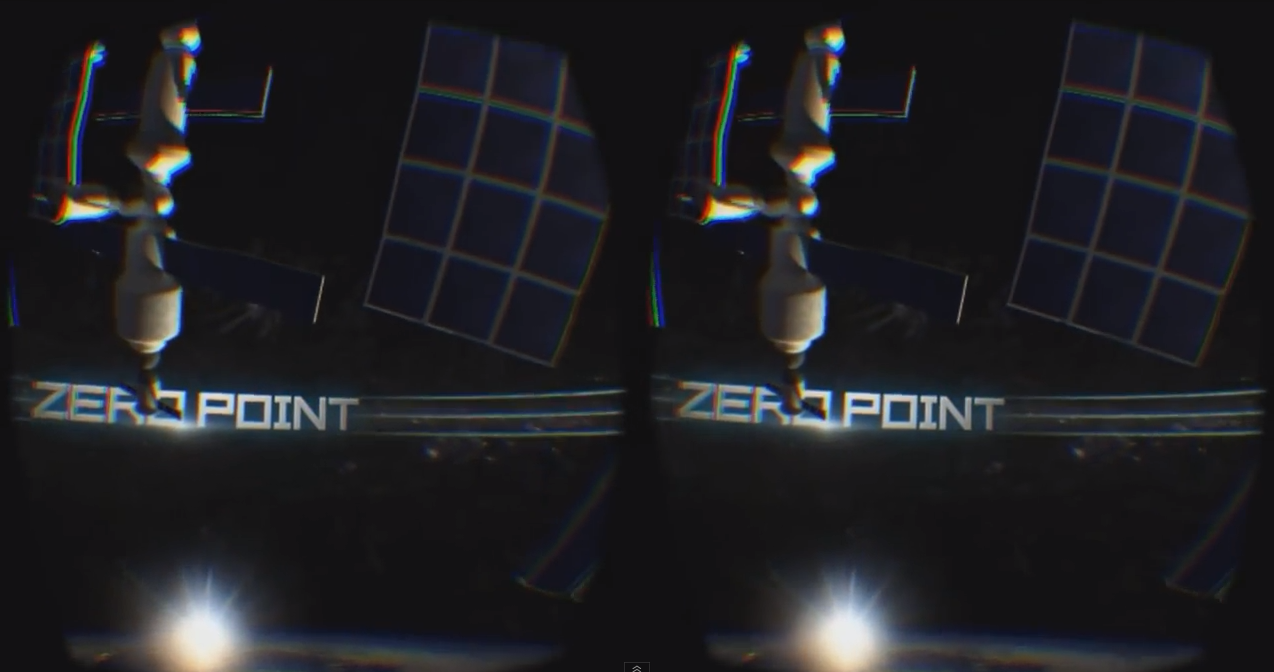
\includegraphics[scale=0.15]{pictures/zeropoint_demo.png}
\caption{Zero Point VR 360 film on Oculus Rift DK2 (source: \href{https://www.youtube.com/watch?v=DsXEUPS2uss}{youtube.com}) \cite{linkzeropoint}}
\label{fig:zeropoint_demo}
\end{subfigure}
\begin{subfigure}{0.49\textwidth}
\centering
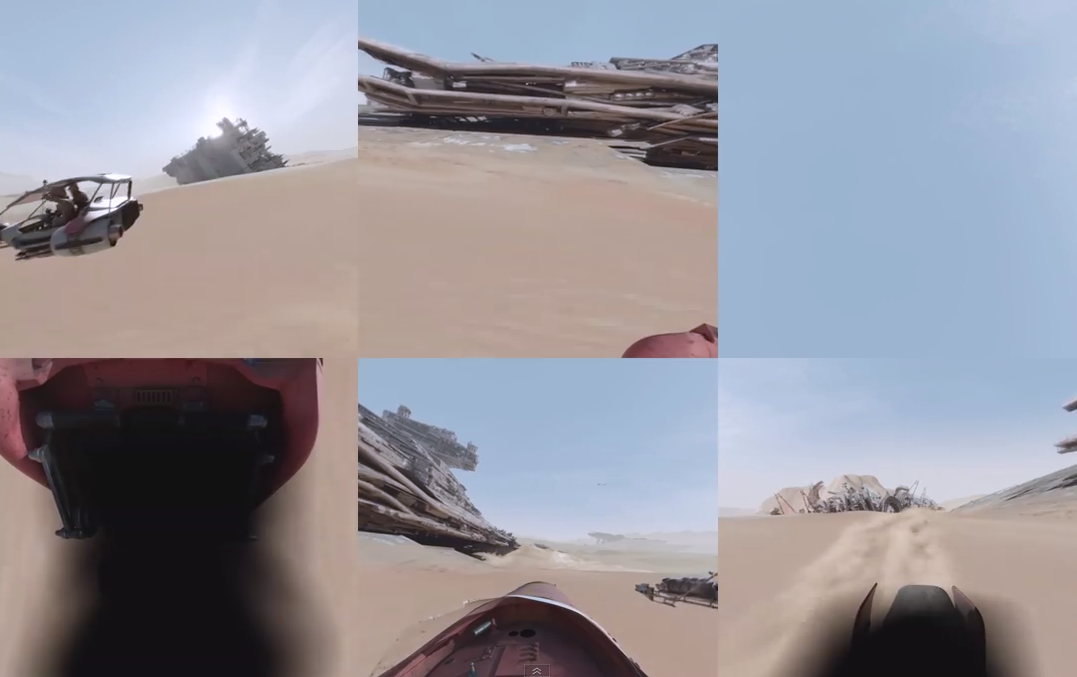
\includegraphics[scale=0.15]{pictures/starwars_trailer.png}
\caption{Star Wars: The Force Awakens Immersive 360 Trailer - different viewpoint screenshots (source: \href{https://www.facebook.com/StarWars/videos/1030579940326940/
}{facebook.com}) \cite{link_starwars_trailer}}
\label{fig:starwars_trailer}
\end{subfigure}
\caption{Two examples of modern union of VR and cinema-like experience}
\label{fig:VR_cinema_examples}
\end{figure}
Current research has been tackling the challenge of what is really immersive and in what ways user experience can be enhanced by means of methods proposed by the previously mentioned doctrines, which stretch from photography and optics \cite{immersivity_film} to computer graphics and parallel computation \cite{immersivity_3D}. At the same time, the more veteran branch of computer vision has been researching how computationally relevant features can be extracted from real world imagery and put use to it by giving machines comprehension of what is happening around them \cite{book_cv}. Such information can finally support also humans in various tasks where imaging devices are involved, but still computer vision does not focus on better ways to deliver it to end users. Recent marriage of computer vision and virtual reality gave birth to Augmented Reality (AR), a step forward on this matter: target applications would provide more intuitive, interactive and integrated human-machine interfaces, coherently with the world observed \cite{ar_intro}.

Less explored is the path where all mentioned features find a place in applications where contact with real world is severed or hijacked and how visual coherence can be enhanced the other way around; the field of studies where human perception is involved can extend its applications from more immersive AR tele-presence \cite{telepresence_intro} to the possibility to actual artificially augment human perception capabilities. In this work we investigate the challenges of immersive AR by means of a stereoscopic, wide field-of-view (referred from now on as "FOV") head-mounted display (referred as "HMD", head mounted display) and subsequent realization of see-through with cameras. A custom built stereo camera rig used to achieve stereoscopic images showing in the headset what is directly in front of the user, proposing a way to eventually alter them and/or extract scene information with classic computer vision techniques. Our implementation proposes a uniform way The scenario introduces many real-world effects including latency, optical artefacts, depth perception and other and mismatches in real and virtual content: our implementation proposes a way to uniformly face those problems, by proposing a processing pipeline oriented to be platform independent and easy to experiment with for both human perception and computer vision algorithms.

In such attempt, we will traverse common aspects of top-notch techniques for human-computer interaction and perception, belonging to the following fields of expertise:
\begin{itemize}
\item computer vision, which covers the techniques for displaying/enhancing images and extrapolating numerical or symbolic information about the real world. Optics and imaging sensors in general are modelled and therefore used to extract that data, which can range from bare geometrical information (such as distances, position and orientation of a camera or known objects in the scene) to more complex pattern recognition;
\item stereoscopy, a collection of techniques addressing the specific problem of creating or enhancing the illusion of depth in images, exploiting principles in optics and human perception. Most methods involve two separate images to achieve this effect. A combination of such techniques and computer vision models opens the door to computer stereo vision, where more than one image is used to extract data, thus requiring less known parameters from the scene;
\item virtual reality, a discipline that implies mathematical models, actuators and sensors to replicate real world experiences in real time in form of entirely computer-simulated environments and give them interaction capabilities. High relevance is given to human psychology and perception limits in order to recreate a lifelike experience. Images are in this case entirely synthetic: models and image enhancements implied have lot in common with computer vision, although the latter focuses on analysis. We find the most common expression of their combination in what is called augmented reality.
\end{itemize}

In the specific we will experiment with Augmented Reality/Virtuality, with a big focus on high visually immersive applications through the use of a virtual reality headset. A custom built stereo camera rig is used to achieve stereoscopic images showing in the headset what is directly in front of the user, proposing a way to eventually alter them and/or extract scene information with classic computer vision techniques. The aim is to study the relationship between real world captured and computer generated images and propose an acceptable solution for their blending.

\section{From Augmented reality to Augmented Virtuality}

As we speak of Virtual Reality environments we refer to an experience in which the user is fully immersed, therefore as much isolated from the real world. The perception of one’s self actually being in a different place gets deeper when involving more advanced sensory to track our movements and proxies like avatars to keep alive what is called in VR the "sense of presence", a critical term that expresses the longing deep connection with user perception and psychology \cite{vr_presence}. However, there are cases where we might want to take full advantage of the high level of interaction with a virtual environment without giving away the connection with the real world. Virtual reality is mainly meant to bring one’s perception in a controlled environment with its own rules, but what if we want to retain all the aspects of the environment surrounding us plus enhancing it with virtual elements? What if we want indeed to be brought in a different place, where everything is real except our own presence?

\begin{figure}
\centering
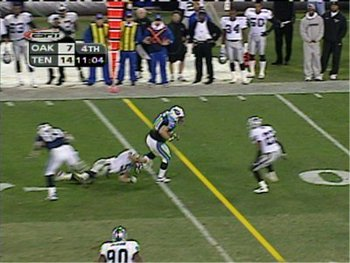
\includegraphics[width=7cm]{pictures/1st_and_ten}
%\caption{This caption is very long \newline ---in fact, it is so long that it doesn't fit on one line}
%\caption
%[1st line \newline 2nd line]
%{\begin{minipage}[t]{.8\linewidth}This is the caption \\This is the second line \end{minipage}}
\caption{The "1st and Ten" system, one of the first successful applications of augmented reality in sports (source: \href{http://www.howstuffworks.com/first-down-line.htm}{howstuffworks.com})}
\label{fig:rugby_ar}
\end{figure}

Augmented Reality explores ways of including virtual elements in the real world. Typically application’s aim in AR (as we will refer to from now on) span from showing additional information to actually place entire objects in the observed scene. The goal is not only keeping intact contact with reality but making it interactive, enhancing it with arbitrary content in the less obtrusive and more intuitive way possible. AR may or may not have reasons to track user pose or actions, but never involves the usage of avatars of any sort, since user is meant to feel exactly where he actually is.

Nowadays, any device that embeds a camera, a screen and a decent processing unit can feature AR applications, whether its computational complexity depends on features extraction \cite{link_google_translate_AR} or no extraction at all \cite{link_IKEA_AR}. However, even though availability and cost of the hardware makes them accessible to anyone, their use is not as much diffuse as one would expect. The reason is to find again in obtrusion and intuition, which brings us to transparency and integration. The real seamless integration between real and virtual is limited by the not-as-integration between individuals and devices; current systems are still far from perfect, and system designers typically end up making a number of application dependent trade off, going from simply info-graphic content such as sport games on TV or HUDs to more immersivity and interaction oriented applications such as medical surgery, complex machinery repair and other tasks that require a specific training.

\begin{figure}
\centering
\begin{subfigure}{0.49\textwidth}    
\centering
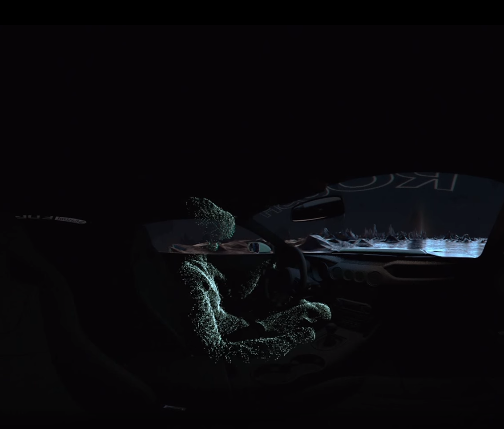
\includegraphics[scale=0.5]{pictures/titanium-a}
\end{subfigure}
\begin{subfigure}{0.49\textwidth}
\centering
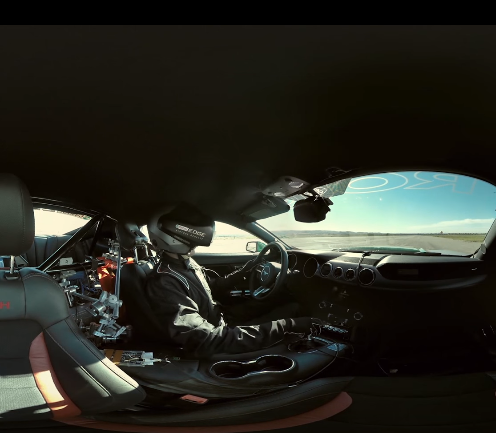
\includegraphics[scale=0.5]{pictures/titanium-b}
\end{subfigure}
\caption{Titanium Strong Virtual Drift, virtual (left) and real (right) view. A very effective example of augmented virtuality (source: \href{https://www.youtube.com/watch?v=WJyG76Izk8M}{youtube.com})}
\end{figure}

On the other hand, some applications are meant exactly for hijacking individual perception, even if not entirely, and carefully control it. That is the case where user is still supposed to interact with reality in some way, but how and when is not up to him. This is the general concept for Mixed Reality (MR), placed midway between pure virtual and real; according to Milgram’s continuum \cite{milgram_continuum}, AR is indeed a form of MR in its most reality-oriented form. Moving towards MR we find quite well-known devices such as night or heat vision goggles: not so far away to require avatar representation but enough obtrusive to completely replace environment as we see it.

As we start to inject into the scene arbitrary information, which is not at all derived from real environment, we cross the boundary of Augmented Virtuality (AV). Roles are inverted: virtual experience can be somehow enhanced with outside information or content. Usually applications of this kind aim to keep contact with real world but also experiment with new ways of representing it. Also the user feels to be somewhere different from everyday world, but still are cases where avatars are not needed depending on the implementation: think for example to tele-operating a humanoid robot, where an avatar is not really necessary if the robot stays in the sight of the user, even better if his "virtual eyes" are on robots head (as in telerobotic surgery \cite{telepresence_intro}. This is not true in tele-presence applications, where real world interaction is mostly perceived as an enhancement of VR experience.

\begin{figure}
\centering
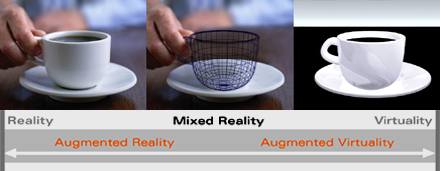
\includegraphics[width=10cm]{schemas/milgram_continuum_enhanced}
%\caption{This caption is very long \newline ---in fact, it is so long that it doesn't fit on one line}
%\caption
%[1st line \newline 2nd line]
%{\begin{minipage}[t]{.8\linewidth}This is the caption \\This is the second line \end{minipage}}
\caption{A graphical representation of Milgram's continuum (from: \href{http://proceedings.spiedigitallibrary.org/proceeding.aspx?articleid=981543}{Augmented Reality: A class of displays on the reality-virtuality continuum})}
\label{fig:milgram_continuum}
\end{figure}

\begin{figure}[h!]
\centering
\begin{subfigure}{0.49\textwidth}
\centering
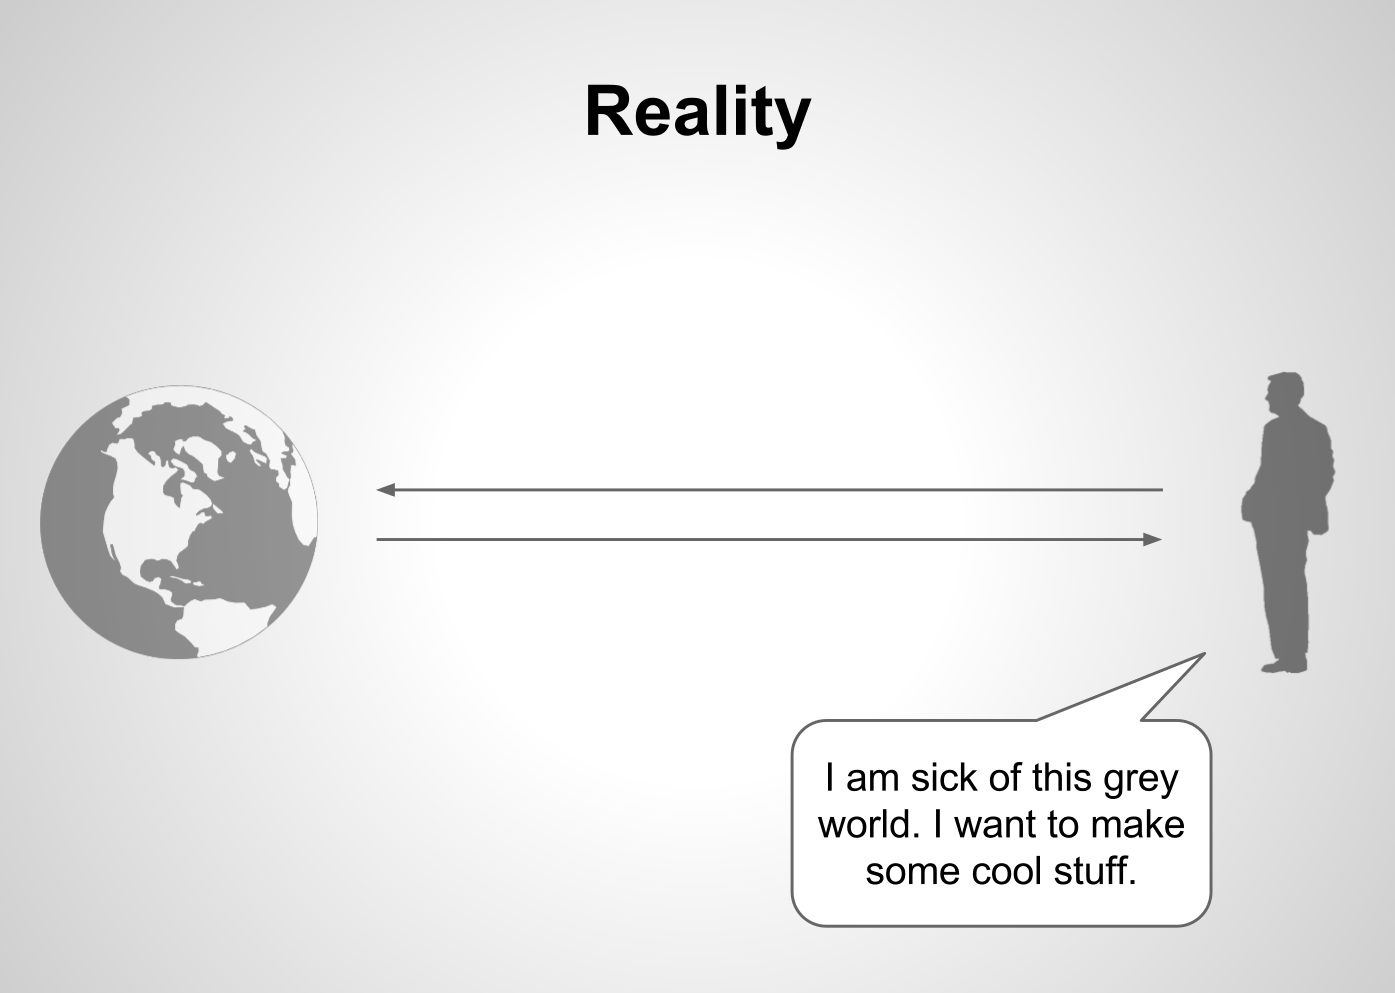
\includegraphics[scale=0.13]{schemas/reality1}
\end{subfigure}
\begin{subfigure}{0.49\textwidth}
\centering
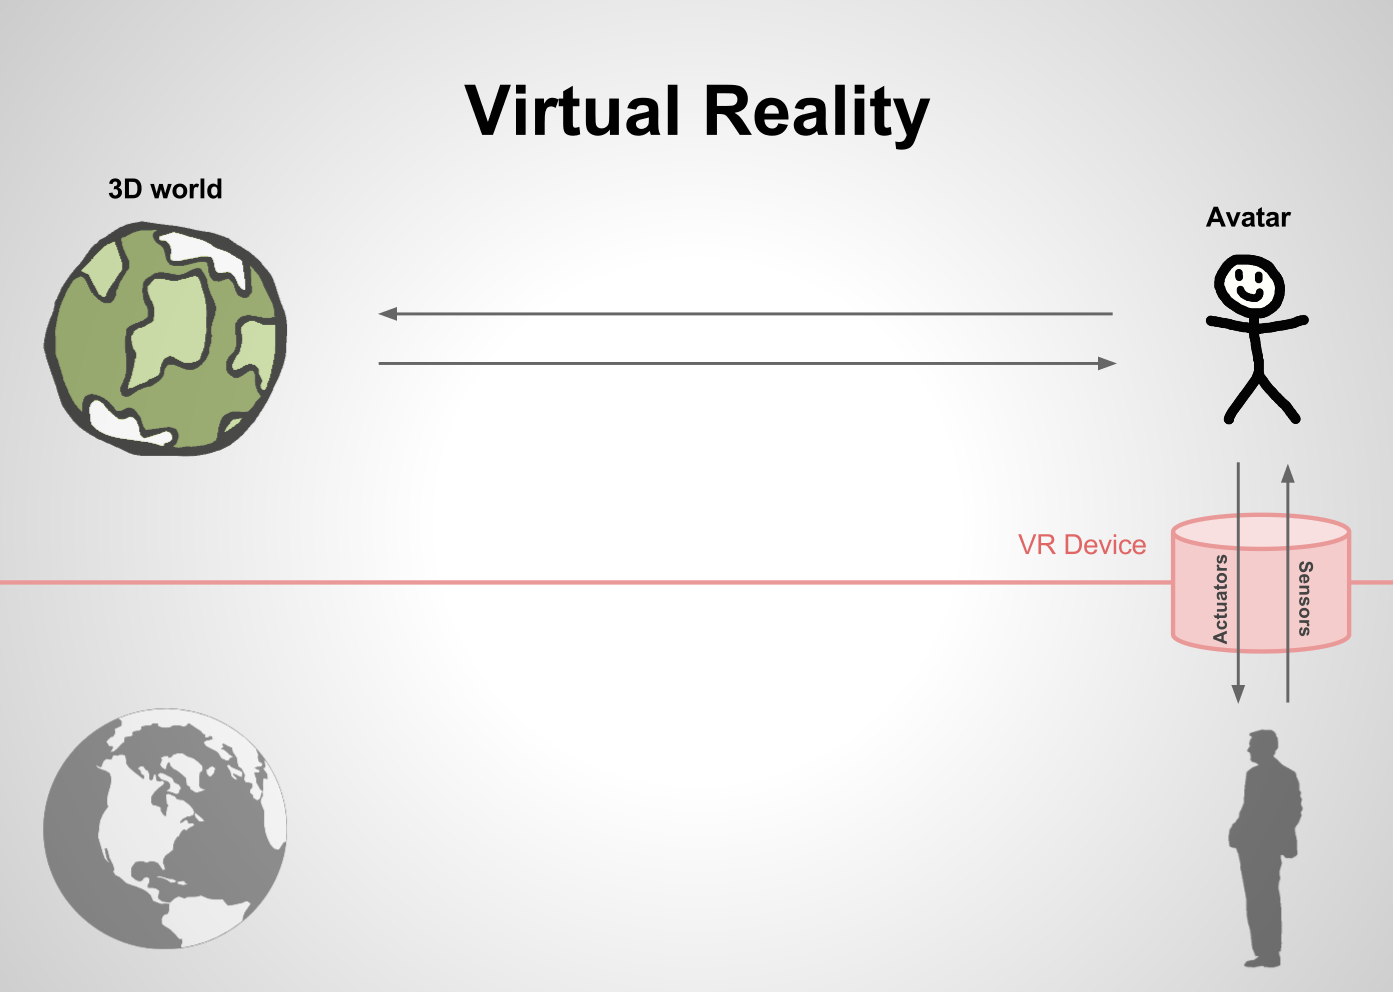
\includegraphics[scale=0.13]{schemas/virtualreality}
\end{subfigure} \\[1em]
\begin{subfigure}{0.49\textwidth}
\centering
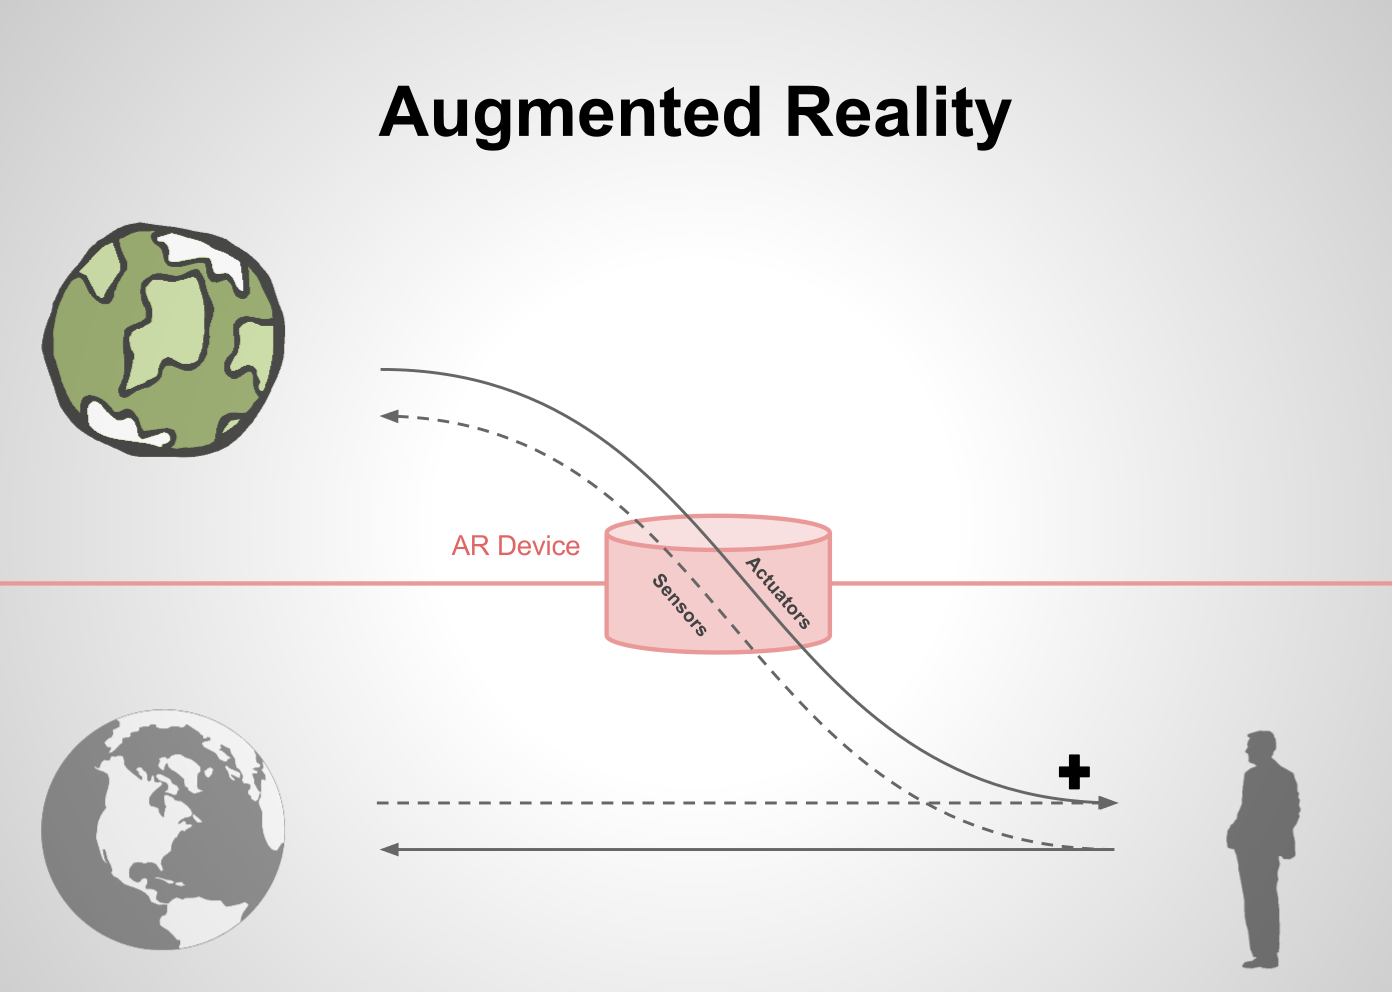
\includegraphics[scale=0.13]{schemas/augmentedreality}
\end{subfigure}
\begin{subfigure}{0.49\textwidth}
\centering
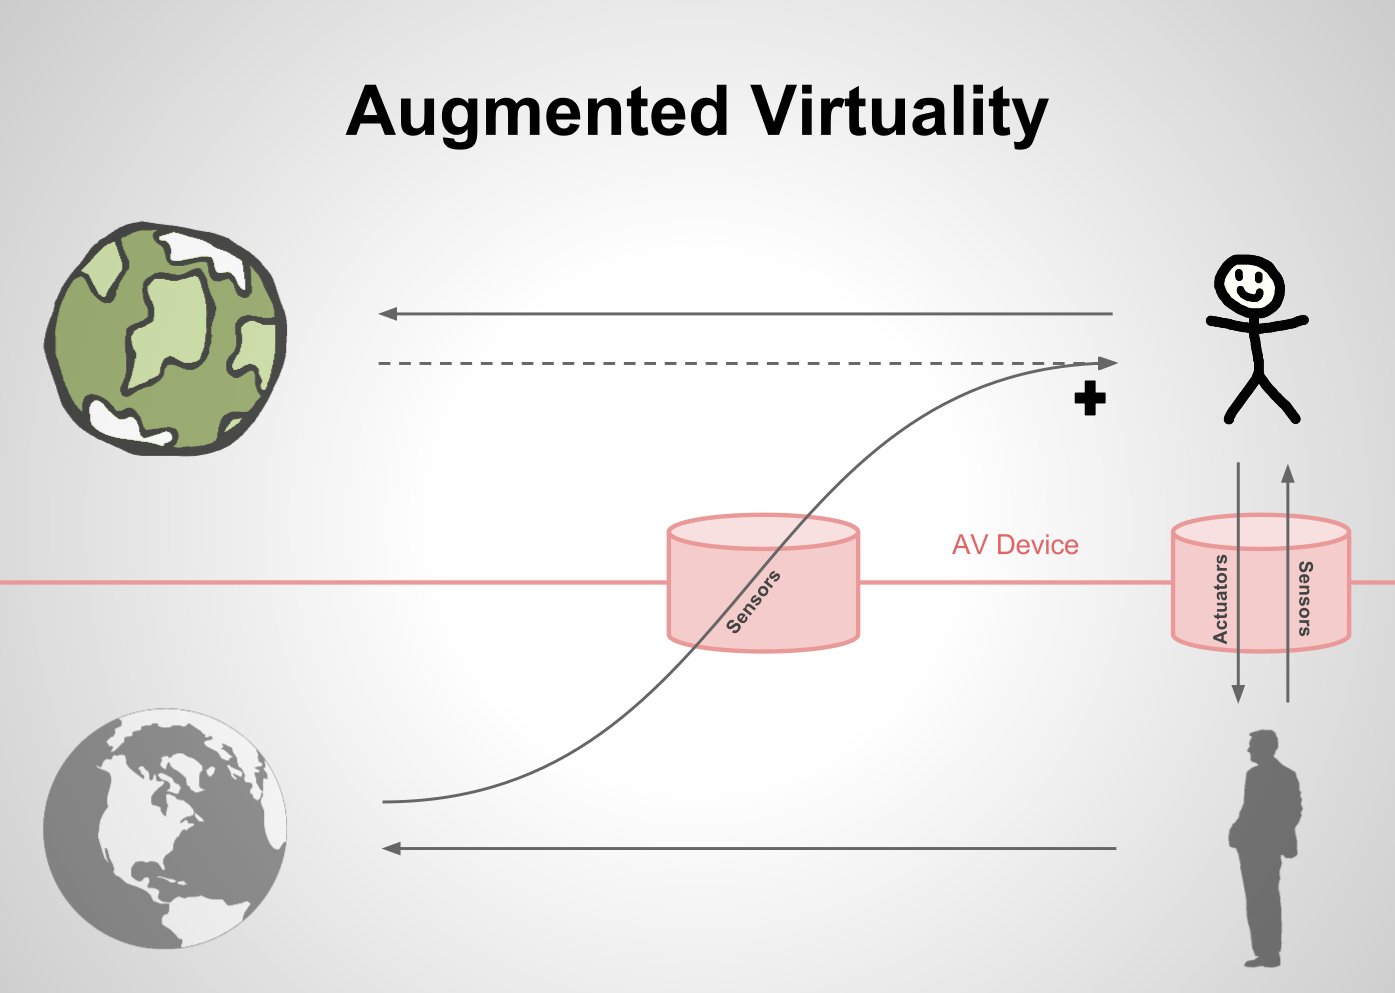
\includegraphics[scale=0.13]{schemas/augmentedvirtuality}
\end{subfigure}
\caption{A simplified overview of mixed reality approaches. Standard arrows picture direct connections, while dashed arrows partial intervention. Their direction indicate the flow of information.}
\label{fig:mixed_reality}
\end{figure}

\newpage

\section{Optical and Video See-through devices} %limits and advantages
Devices offering a very good compromise between interactivity and transparency for AR/AV immersive applications are Head Mounted Displays (HMD), where images are projected directly in the user’s view. HMDs often include on-board sensors like gyroscopes and accelerometers or simply passive markers like US or IR to keep track of head position, orientation and speed so that images can be displayed accordingly \cite{tracking_AR}. As for the displaying part, two systems design have been proposed: video and optical see-through. Both have as image sources real and computer-generated world, but end up to be very different for technical reasons. In a work of Rolland-Fuchs \cite{optical_vs_video_st} a comprehensive taxonomy of video and optical see-through technology is given, through which we will now describe background and motivate the choice of our work.

A video HMD with no images from the real world is common in VR applications: its ability to block out the real world view thus cover the highest user’s field of view with the crispiest computer-generated image possible. Adding on-board image capture capability it can be considered a video see-through device, capable of both AR/AV applications. Experimenting with AV has virtually no limits, since other kind of sensors or even more cameras may be involved to show something different to the user, as soon as a good level of immersion is guaranteed. The same cannot be said for a canonical AR application: captured images should appear as close as real and feel natural to the user, suspending his instinctive disbelief that what he is seeing is not real. A series of optical limits come in play that simply cannot be surpassed by a simple screen, which is just a simplification of how images are perceived by the human eye. To address this lack, the most pursued strategy is providing additional hints to the brain by involving head motion and even eye gaze tracking to act on image behaviour. But even if a good compromise can be reached, it cannot be considered acceptable in the long run: human brain is as good at noticing imperfections as adapting to them. This constant effort generates an increasing amount of stress in the user that, depending on the subject, may experience from simple eye strain to temporary sickness \cite{virtual_sickness}.

Optical see-through devices systematically solve the problem, providing semi-transparent lens or screen that lets light in while computer-generated images are merged through a set of mirrors. The connection with reality is kept nearly intact, therefore no perception side-effects are present as soon as device is perfectly calibrated. The limit of optical HMDs is only technological. While they are the best option for AR applications, they still lack the capability of showing environment as only a completely transparent glass would allow or virtual content as only a completely opaque screen would do. Moreover, there is always a discrepancy between overlay (region where virtual and real information are superimposed) and peripheral FOV of the user, an issue video HMD not really have since everything else from the screen is blocked out. Cost and build limits still not allow to cover high field of views such as ones achieved by recent video counterparts like Oculus Rift \cite{oculus_rift}. In other words, optical see-through solutions are promising for a variety of applications whose working space is within arm reach and require reliability and minimum distraction. Even with the best performance possible, a video see-through headset can be dangerous in situations where seeing what is going on is vital.

Optical HMD is so far the candidate to be more present in everyday life in the future. As we already mentioned, its current obtrusive nature makes it hard, but recently a lot of effort has been spent in this direction. "Light" versions of optical HMD can be identified in early commercial products such as Google Glass \cite{google_glass} or the still unreleased Microsoft Hololens \cite{microsoft_hololens}, whose aim is supporting multi-purpose applications to supposedly revolutionize man-machine interfaces.

As for video HMD, it is still very used in VR and tele-presence/tele-operation applications \cite{telepresence_intro}. The current work has its starting point on its limits and possibilities. We found its features to be best for experimenting with different media and 3D content where integration with reality is a possibility not a necessity. Our aim is to build a basic AR video see-through setup that can allow users to experience both VR and AR seamlessly, with a constant focus on code reusability for future technology development (that will eventually overcome limits of both optical and video HMDs) and researchers to deeper understand their connection in human visual perception.


\begin{figure}
\centering 
\begin{subfigure}{0.49\textwidth}
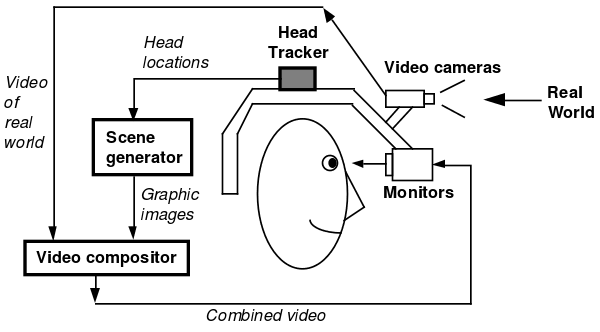
\includegraphics[width=\linewidth]{schemas/videoST_hmd}
\end{subfigure}
\hspace{\fill}
\begin{subfigure}{0.49\textwidth}
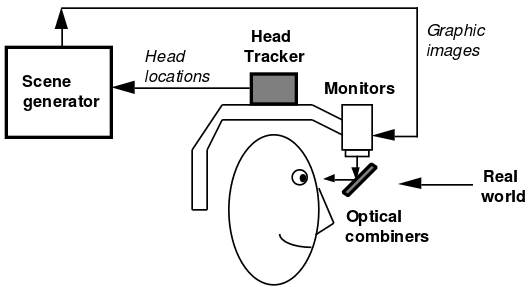
\includegraphics[width=\linewidth]{schemas/opticalST_hmd}
\end{subfigure}
\vspace*{0.3cm} % (or whatever vertical separation you prefer)
\begin{subfigure}{0.49\textwidth}
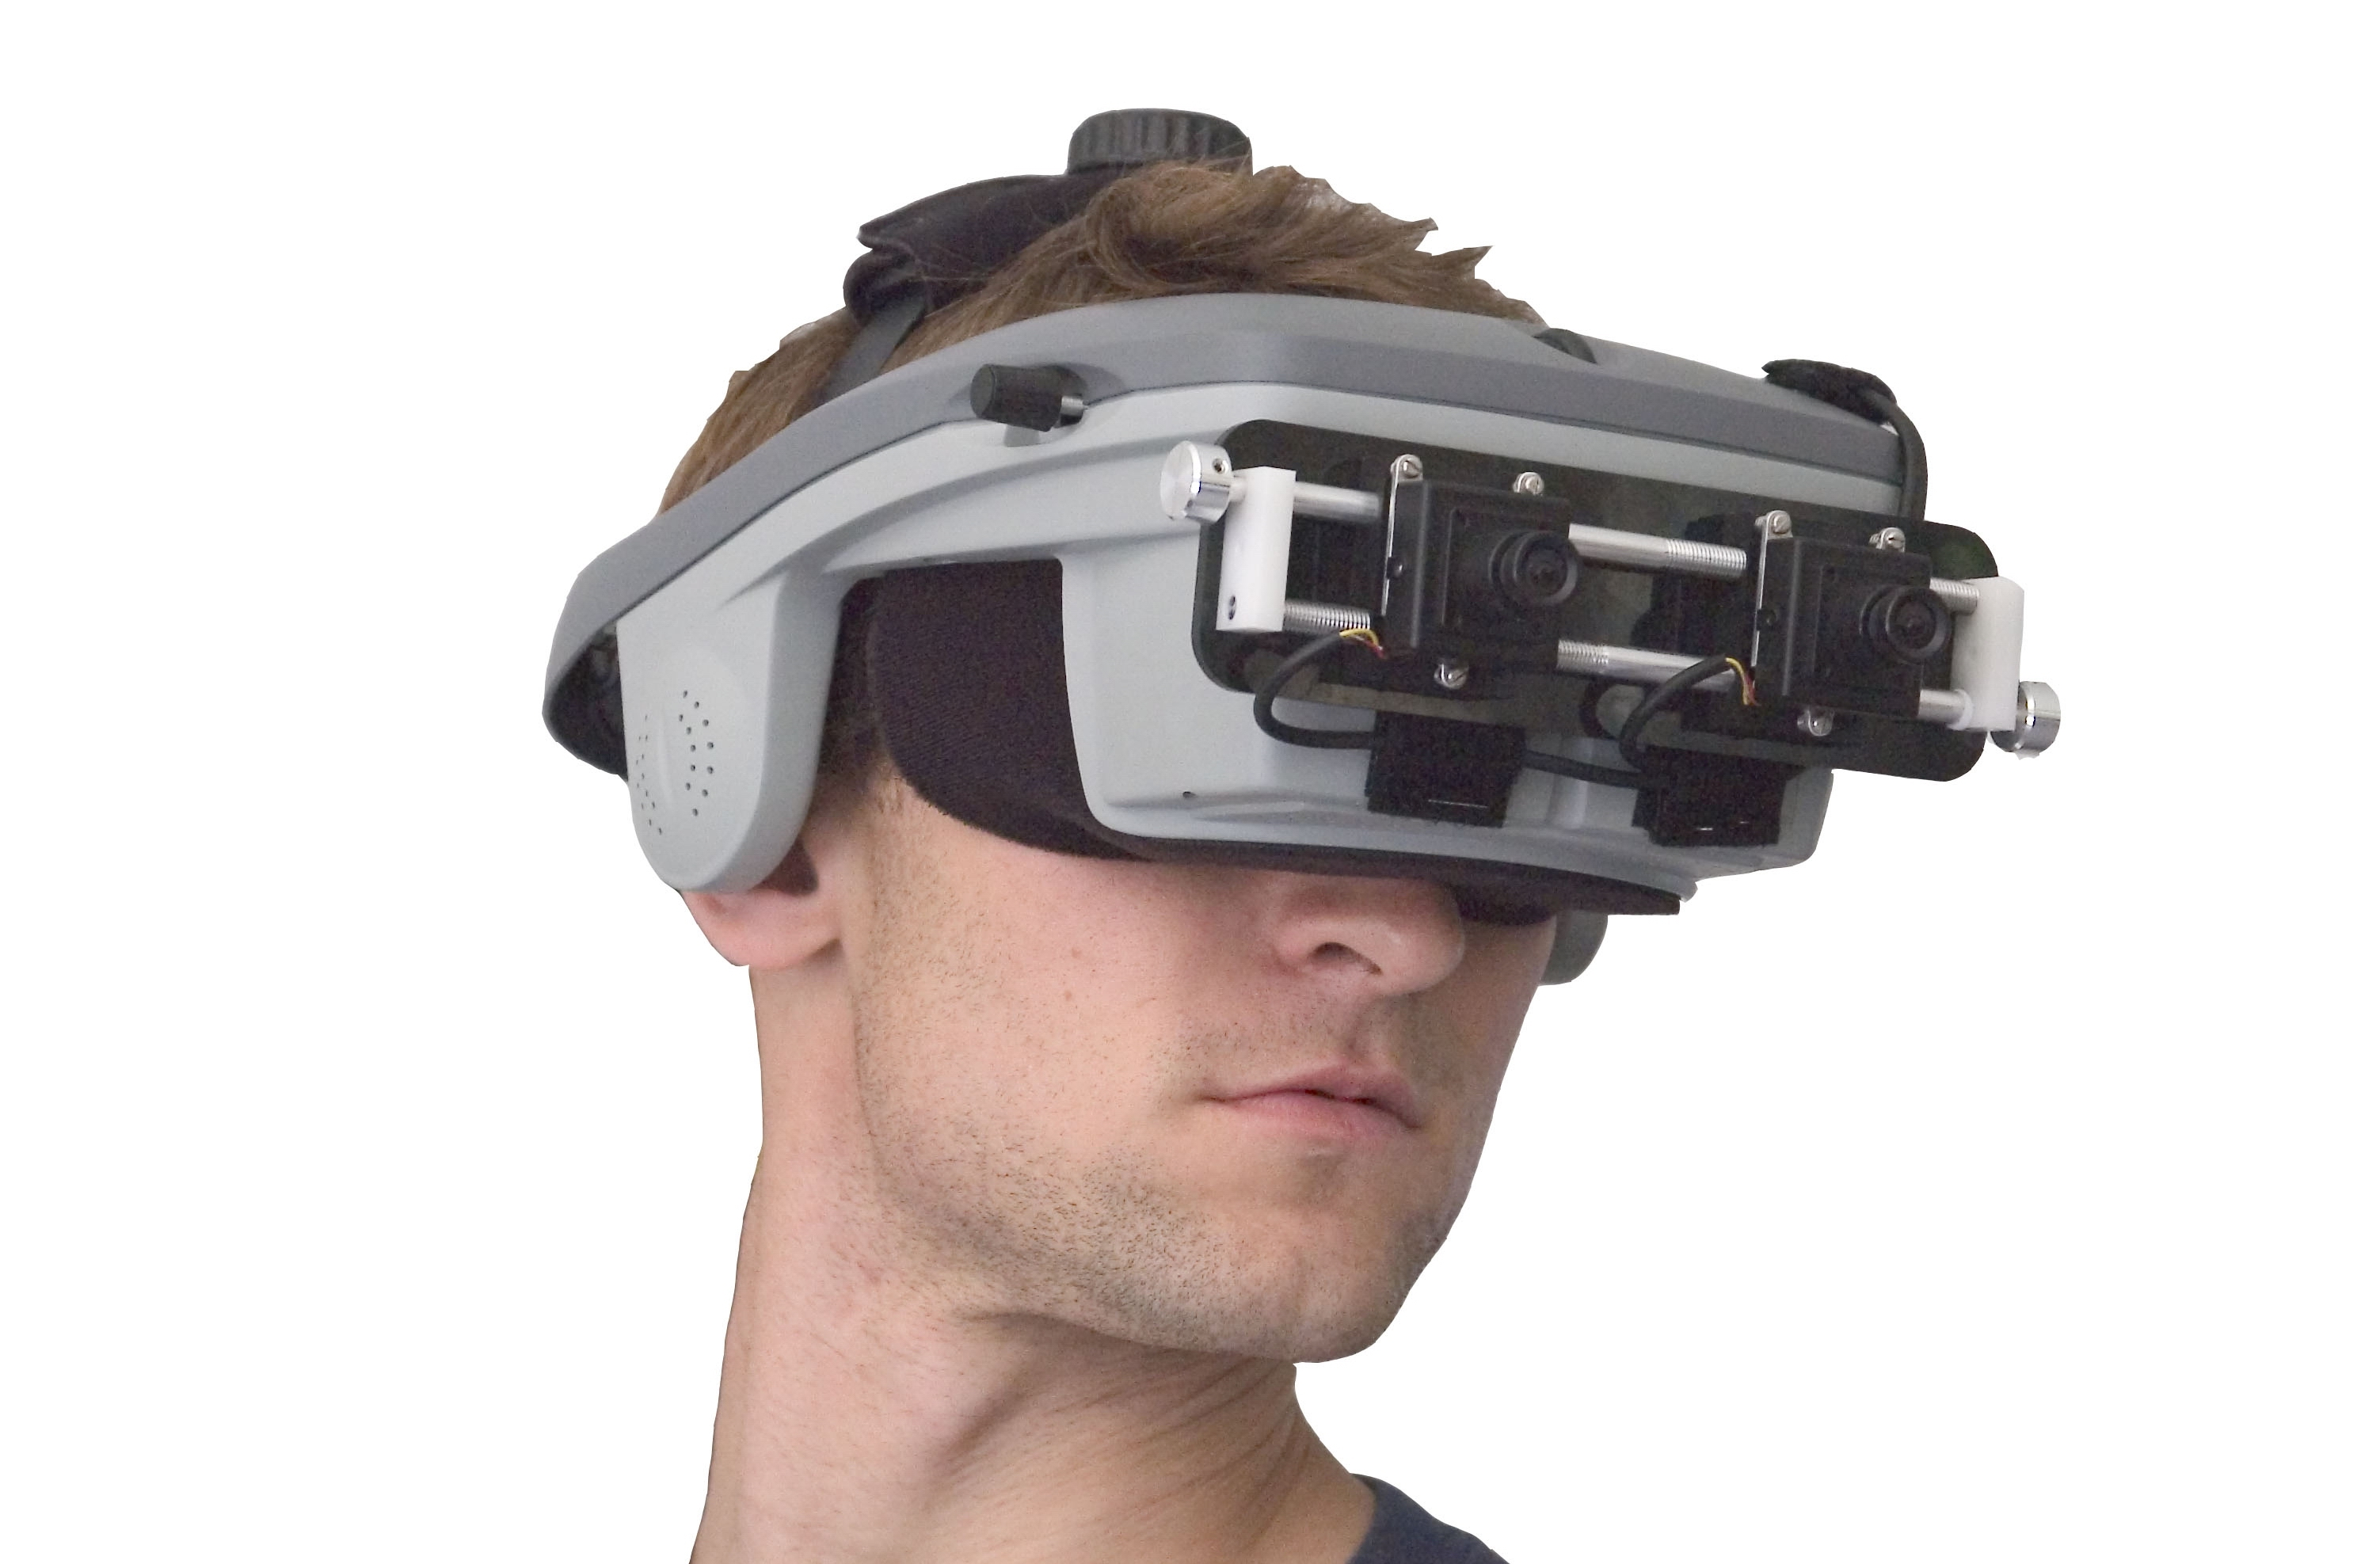
\includegraphics[width=\linewidth]{pictures/videoST_example}
\end{subfigure}
\hspace{\fill}
\begin{subfigure}{0.49\textwidth}
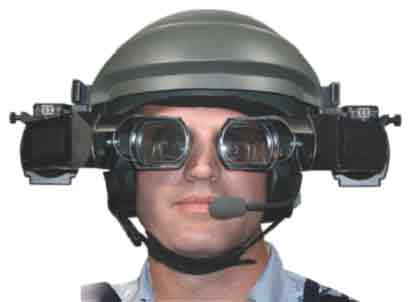
\includegraphics[width=\linewidth]{pictures/opticalST_example}
\end{subfigure}
\vspace*{-3mm}
\caption{A video (top-left) and optical (top-right) see-through HMD conceptual diagram comparison for AR (source: \href{http://www.cs.unc.edu/~azuma/ARpresence.pdf}{A Survey of Augmented Reality}). At bottom two respective examples, WorldViz VideoVision powered HMD (left) and Simeye XL100A (right).}
\label{fig:video_optical_seethrough_comparison}
\end{figure}

\section{Perceptual goals and technical issues}
\subsection{High field of view}
As said, immersion in general depends on factors that allow user experience to be as close to real world perception as possible. FOV essentially limits head movements of the user, who can simply gaze at objects he manipulates in the natural way he is used to in everyday life. Restricting a person’s FOV, in fact, has been shown to affect people’s behaviour and degrade task performance \cite{restricting_FOV}. With the advent of modern VR HMDs, we cannot exempt from classifying high FOV as a concern. Though is not really necessary for a variety of applications, neglecting the full potential of recent hardware is to be considered a waste. Oculus Rift had its strong points on high FOV and low latency and is on the verge of releasing a product for the masses. For a VR/AR application, it will be required not only working at high frame rates with high image angles, but also filling discrepancies between virtual and real captured images. Even though user may adapt to one image with scale different from the one he is used to, he would not be able to (and must not be required to) decide between two. Apart for custom built solutions, FOV in HMD and camera never happen to match perfectly, so this must be kept in mind. This is a consequence of specific hardware implementations.

\subsection{Minimum distortion and high resolution}
Digital (as resolution) and optical (as distortion) per-device limits come in play, as technical and not perceptual issues like FOV discrepancy. All HMD setups involve a specific setup of mirrors/lenses and a consequently adequate screen/projector to get the image just right, no matter if optical or video. Resolution is a problem that is on the way of being solved with the advancements in displays, projectors and GPUs industry. Application is not really dependent on that except from the amount of computational load to be generated. By increasing FOV, resolution becomes more critical, as image dots must be spread across a wider area.
For high field of view HMDs, lens distortion and chromatic aberration are not negligible. "Undistortion" (a slang term indicating the distortion correction process) has to be performed in the rendering pipeline prior to visualization for both virtual and real image.

\subsection{Real and virtual perception discrepancy}
We already mentioned the need of matching FOV as a perceptual issue, way more noticeable when working with high angles. We classify under perceptual discrepancies all issues that would most likely destroy immersion. Dealing with an AR application with a video HMD, we focus on reaching the best possible imitation of what would offer an optical setup. Stereoscopy affirms that a stereo rig can provide binocular parallax, so that depth perception can be reached for both virtual and real objects. Moreover, raw depth information can be extracted from the real scene and simulate occlusion between real and virtual objects \cite{GPU_accel_stereo_AR}.

While this is feasible in practice, geometric problems keep us apart from delivering the desired effect to the user: a virtual object (detected or entirely generated) is placed in a 3D environment and its projection can be rendered relative to user's view position/orientation; a real scene image is instead already a projection from camera point of view and should in theory match with the virtual one. A good trick is to use mirrors, so that camera optical path reflects overlaps with eye's, even if in a different position \cite{optical_vs_video_st}. This solves the issue but at a great cost: camera FOV is sacrificed due to the path between the mirrors and is also the reason why optical see-through have this limit in the first place. When high FOV is a requirement and no mirror is involved, user is assumed to adapt to the shifted viewpoints of the cameras, so cameras are supposed to be placed as close to the eyes as possible.

The main perceptual limit for video and optical see-through is depth of field reproduction: while video HMD can only offer a geometrical simplification of real stereo image (since real cameras cannot be placed where eye pupils are) which is not a problem for the optical counterpart, simulating virtual stereo troubles both. This is because screens and projectors reproduce images on a flat surface at a constant distance from the observer, on which each eye has to focus on to get the image crisp. This is not really a problem when one non-stereo image is presented in front of both eyes since it is recognized flat as it is (like whatching a tv). As soon as stereo comes into play, objects can be moved and be perceived behind or in front of that surface and the brain will eventually ask extraocular muscles to converge eyes but also iris to focus to that (virtual) converging distance; light reaching each eye still comes from the actual screen, so there will be a discrepancy between eye convergence and expected focus distance, introducing strife and in the worst case object will still appear blurry. This is why, with current technology, it is good practice to place the display surface at the expected average working distance \cite{stereo_rules}, or at infinite if that is not known in advance where presumably there is minimal eye strain. This aspect is essentially independent from software VR/AR implementation and can be only partially countered (we will discuss such work-arounds in the next chapter) so we can only feel confident that this hardware limitation will be overcome in the near future (lightmapping technology \cite{light_field_mapping} and the to-be-unveiled "Magic Leap" project \cite{magic_leap} in Figure \ref{fig:magic_leap}).

\begin{figure}
\centering
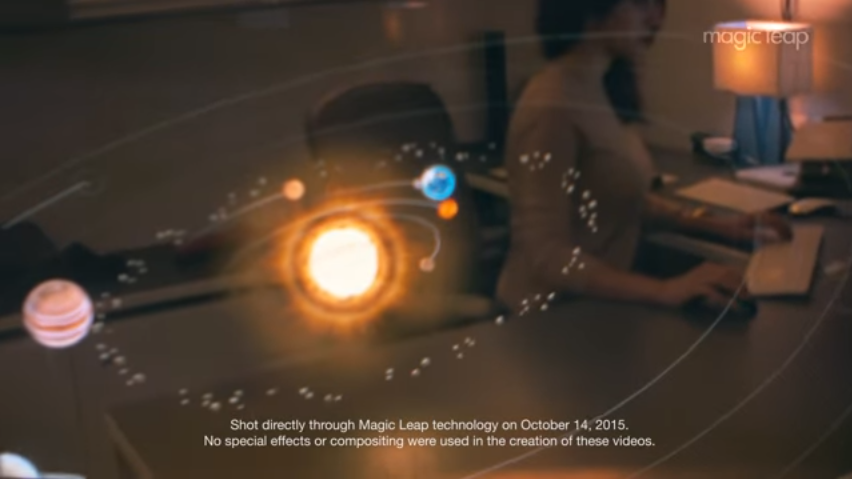
\includegraphics[width=13cm]{pictures/magic_leap}
\caption{What should look like through Magic Leap technology \cite{magic_leap}, without the use of special effects or compositing. Note how virtual objects get in/out focus coherently with real environment (source: \href{https://www.youtube.com/watch?v=kw0-JRa9n94}{youtube.com})}
\label{fig:magic_leap}
\end{figure}

Other discrepancies regard detail of virtual objects, such as shadow and lights and realistic texturing. Users can still distinguish between a real object and its virtual counterpart depending on the fidelity with which it has been reproduced. This however depends on developer's choice: one may want to represent a real world augmented with evident digital cues (in order to keep user conscious of what is real and what is related to what is real) or focus on trick users in thinking all he sees is real (or vice-versa all is virtual). Our efforts in reducing discrepancies perception will concentrate on keeping whatever real or virtual content consistent with whatever scene is shown on screen. This goes for perfectly overlap virtual and real worlds and, as an eventual future development stage, their deeper interaction with depth mapping.

\subsection{Performance limitations}
Fluent image rendering is the sine-qua-non for all previous conditions and can be achieved with reasonable (in gaming, 60 fps is considered the ideal standard) frame rate by any good 3D engine and satisfactory hardware for a VR-only environment. 3D graphics computation are exceptionally fast with dedicated GPU, but still require a good CPU for sequential operations. As we approach to computer vision applications, high parallelism is a desirable factor but nothing a modern CPU cannot handle for 2D computations (such as image undistort, object detection and so on). In VR/AR application, vision and rendering must then act in parallel and in real-time.
\iffalse
\\
TO EDIT\\
Other than disposing of top-notch hardware, there are a few rules of thumb to follow:
- lower image resolution: this would reduce computational load substantially. Always consider hardware and human limits unnecessary high quality settings.
- reduce frame rate: same considerations made above.
- simplify rendered scene (3D only): (to change) keep virtual objects at minimum number/complexity, crop them out if not visible again for limitations.
- 2D image elaboration through 3D hacks (to change)
- implement algorithms with OpenCL/CUDA: specific languages are available to parallelize custom operations on highly parallel hardware, but requires specific knowledge and dedicated implementation.
- run serialized code when CPU should be waiting for GPU\\
END EDIT\\
\fi
However, no matter what, inevitable to hit is the wall of "system latency", which refers to the time gap between a new set of data is retrieved from a sensor and the correspondent synthetic image is fully rendered. Since this exchange can be instantaneous only in theory, such physic limitation cannot be simply solved by more powerful hardware. In VR/AR applications, software "hacks" can be used to tighten the gap enough to trick the brain, as we will see. Moreover, since measure data belong to different natures, different non-synchronized devices working at different data rates, lag problems will be faced separately. 

\section{Document outline}
In the introduction we have provided a motivations for experimenting with AR on a video see-through HMD and a fast glimpse of the problems we will have to face in the following dissertation. In chapter 2, we will run deeper through aspects critical for understanding the options and state-of-the-art tools our work will exploit to tackle such problems. Once an overview for both reality and virtual reality has been given, we will focus on the proposed methodology in chapter 3, combining and pushing forward what presented in chapter 2. In chapter 4 and 5 we offer our technical results on tests performed and a conclusion opening to future developments and works.

\chapter{Related work and state of the art}

\iffalse
\section{Camera modelling fundamentals in computer vision}

\subsection{Pinhole camera}
\subsubsection{intrinsic parameters}

\subsection{Lens distortion correction and camera calibration}
\subsubsection{distortion parameters}
\subsubsection{extrinsic parameters}

\subsection{Fish-eye camera}
\fi

\section{Solutions for stereoscopy}

In this paragraph, we attempt to analyse modern approaches to reproduce depth cues using stereo cameras. Additional hints will be given to better understand how such configurations can impact on computation-based depth information extraction with stereo computer vision, thus encouraging its employment as a direct consequence of this work.

\subsection{Stereopsis}
Depth perception may arise from a variety of depth cues, most of them related to a scene viewed by a single eye. These go from motion parallax to simple size differential, but we will not focus on those. What really stereo imagery focuses on is delivering the additional binocular cues, like "stereopsis" and "convergence". Stereoscopy uses two images of the same scene obtained from slightly different angles to do the trick. This is not just an intuitive guess: binocular parallax is what our brain uses to extract image disparities and do its best to estimate real objects distances in our sight \cite{disparity_depth}. Being able to reproduce depth perception in an individual means to be able to recreate those disparities (stereopsis) and consequently make his extraocular muscles contract (convergence).

Assuming null distortion, a stereo vision system can be described \cite{book_cv} with the following parameters:
\begin{itemize}
\item the two camera intrinsic matrices, their aperture and focus distance;
\item their position and orientation in space defined by origin and optical axis; their separation and yaw angle is mostly relevant for stereoscopic effect;
\item epipolar lines and plane, given a chosen point in space within both frustrums.
\end{itemize}
Through these we will briefly describe most used configurations for stereo vision today and what they involve in terms of perception and practical implementation.

\subsection{Stereo rig configurations}

\subsubsection{Parallel cameras}
The very basic configuration is to place two cameras next to each other with their optical axis parallel: line connecting camera origins (baseline) and epipolar lines are parallel for every chosen stereo pair \cite{stereoscopic_3D_acquisition}. In theory this is enough to give the horizontal disparity we are looking for, but is also where imaging devices meet their limit. Stereo pairs, which are the pairs of points of the scene whose projection is visible in both images, can be found only in a portion of each frame, which corresponds to the portion of the scene visible by both cameras. This means that left-most part and right-most part of left and right camera respectively won't offer useful stereo information \cite{correct_stereo_pairs}. This is much like what happens at the edges of our eyesight, angles that only one eye at a time is able to see. Although those areas don't contribute to stereopsis, it is still what enables us to get such high FOV and the perception of being in the middle of the scene. It is not a case that this helps to achieve good immersion in VR simulations, since user is less forced to rotate his head to explore the environment and can gaze around like he is used to.

More than merely collect horizontal disparities, we want to have also control over the natural convergence effect. For a spherical imaging device such as the human eye, the disparity is expressed in terms of visual angle, while a flat sensor of classic cameras (obeying to pinhole model) can instead be seen as the limiting form of a spherical sensor with an infinite radius of curvature \cite{camera_convergence}. This means that an inward rotation of the sensors may do indeed the trick. However in stereo computer graphics parallel-type setup is very common for representing each eye with a virtual camera: the reason is that most of the times where the user is supposed to focus is not defined and dedicated sensors and algorithms are needed to track eye movements to simulate it properly \cite{dynamic_virtual_eye_convergence}. For the parallel stereo configuration, convergence can then be adjusted also by a translation of the cameras parallel to sensor plane or alternatively a translation of the image on the display, if this happens to be a flat surface \cite{camera_convergence}. By shifting displayed frames on the screen we can control depth of the objects percieved by the observer, that will be seen in front (negative parallax) or behind the screen (positive parallax). The screen plane is coincident with what is called zero-parallax plane. With no shifting, zero-parallax plane is placed at infinite and every object is perceived in front of the screen.

\begin{figure}
\centering
\begin{subfigure}{0.32\textwidth}
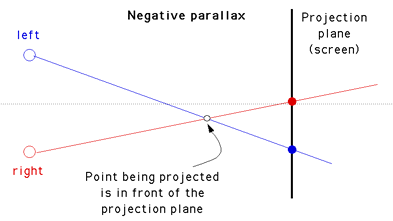
\includegraphics[width=\linewidth, height=3.5cm]{schemas/negative_parallax}
\end{subfigure}
\hspace{\fill}
\begin{subfigure}{0.32\textwidth}
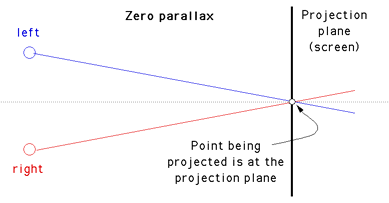
\includegraphics[width=\linewidth, height=3.5cm]{schemas/zero_parallax}
\end{subfigure}
\hspace{\fill}
\begin{subfigure}{0.32\textwidth}
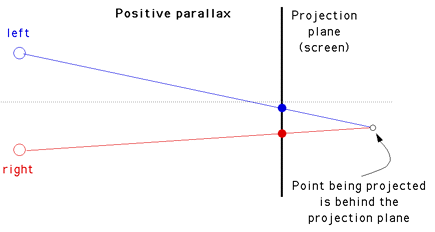
\includegraphics[width=\linewidth, height=3.5cm]{schemas/positive_parallax}
\end{subfigure}
\caption{Different parallax situations. Courtesy of Paul Burke's work (source: \href{http://paulbourke.net/stereographics/stereorender/}{paulbourke.net}) \cite{stereo_pairs_cameras}}
\label{fig:parallax_plane}
\end{figure}

A practical problem with shifting the displayed images on screen is that part of each half-image falls off the boundaries of the screen, therefore losing precious FOV the more we move objects behind the screen. This is also why parallel-type is much used in computer graphics, where it is not a problem to customize virtual camera parameters to cover a higher portion of the scene from the beginning with zero cost.

\begin{figure}
\centering
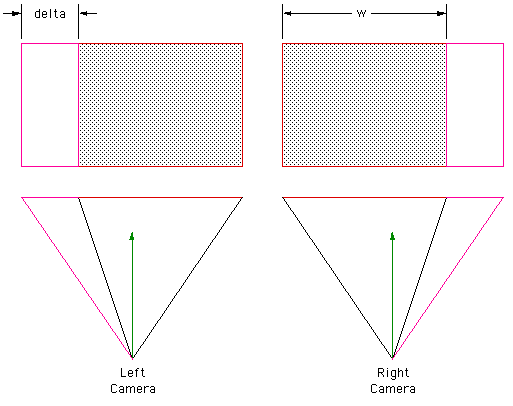
\includegraphics[width=7cm]{schemas/parallel}
\caption{The problem of shifting and losing portion of each image. Paul Burke gives a good formulation of this problem in \cite{correct_stereo_pairs} (source: \href{http://klee.cittastudi.di.unimi.it/~dan/PGL/doc/articoli&libri/CalculatingStereoPairs.pdf} {Creating correct stereo pairs from any raytracer})}
\label{fig:parallel_cameras}
\end{figure}

Also, having most of the scene behind the display is preferred situation in stereoscopy. Having much of the scene too far from the zero-parallax plane causes a disruption of the natural synergy between vergence and accommodation for most users (since objects are not where each eye focuses on). Different reasons make behind-the-screen philosophy a preference: something coming out from the screen more likely will cross its boundaries and will screw up occlusion perception; targets far away are more likely to be on focus together with the screen than closer ones.

\subsubsection{Off-axis cameras}
A real camera can be hacked so that it gets all advantages and simplicity of parallel-type configuration without giving away FOV. Instead of shifting display frame afterwards or translating cameras taking the risk of unnatural results, we can play with sensor/lens alignment. By shifting the sensor in respect to the lens, we can decide the actual convergence angle exploiting all available sensor area. What happens is that camera frustrum is no longer symmetric and allows us to cover different areas of the scene without rotating the lens/sensor. This method is also called shifted-lens or skewed-frustrum stereo and is the ideal way of capturing/reproducing stereo pairs \cite{offaxis_frustrums}.

\begin{figure}
\centering
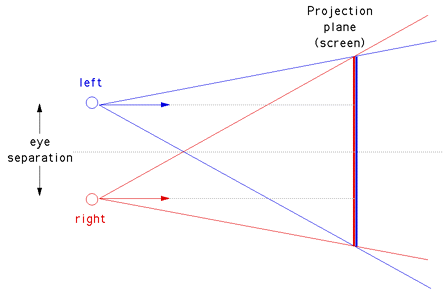
\includegraphics[width=7cm]{schemas/offaxis}
\caption{The image shift is no longer necessary if the view frustrum is shifted by the needed amount}
\label{fig:offaxis_cameras}
\end{figure}

Unfortunately, such vision systems are not very diffused and are difficult to realize in practice due to the high precision needed. Moreover, vergence angle is something to be decided in advance, leaving each device tied to a specific scene and screen target. This is why existing systems of this kind provide adjustable lens/sensor shift and are much more expensive and therefore uncommon.

While this effect is hard to achieve in practice, it can be expressed by the pin-hole model (by means of Principal Point Offset position, not centred). However, in 3D graphics world (where cameras could be entirely customized) still many applications don't go beyond the standard virtual camera model, which as we will see is described by focus point, view and up vector and FOV. A virtual camera matrix (as we will see in chapter 3, its "projection" component) is determined by those parameters even though it is possible to entirely customize it to get the desired frustrum.

\subsubsection{Toed-in cameras}
Optical axis in toed-in configuration converge and baseline intersects with the two camera projection planes (epipolar lines are no longer parallel, but their orientation depend on the stereo pair). As we introduced the convergence problem in parallel-type configuration, we mentioned that rotation of the sensor is a way to go. In reality, this is the pursued option in most cases for image capture \cite{link_toein_diffused}; the reason is its low-cost implementation, plus a decent approximation of what an off-axis setup would offer.
\begin{figure}
\centering
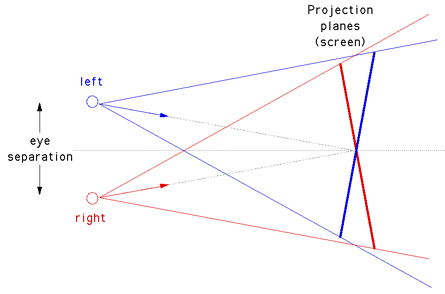
\includegraphics[width=7cm]{schemas/toein}
\caption{Toe-in configuration approximates the off-axis solution by rotating the whole camera body}
\label{fig:toedin_cameras}
\end{figure}
The whole FOV of each camera is indeed preserved and the yaw of each camera can be easily adjusted at capture time. The fundamental problem is that while toe-in stereo makes sense intuitively (as our eyes rotate inwards when we focus on nearby objects), this does not correspond to how 3D is shown. Captured frames are in fact projected into a screen and not differently to each retina. The whole assumption that the image will be displayed on a display orthogonal to viewer's direction (as happens for single camera captures) is still considered valid in 3D movies where there are actually two viewing directions projected into the same plane. This leads to the effect known as "keystoning": artificial vertical disparity is introduced, increasing towards the edges, causing a breakdown of the 3D illusion \cite{link_toein_diffused} \cite{camera_convergence}. Even in less severe scenarios where brain is flexible enough to adapt, it will eventually lead to eye strain, not to mention the already present accommodation/convergence conflict. Since this effect is noticeable at the edges, strategies like artificially reduce the amount of eye separation and keep objects, and therefore the viewer's eyes, in the center of the screen may address the symptoms but not the cause.

\begin{figure}
\centering
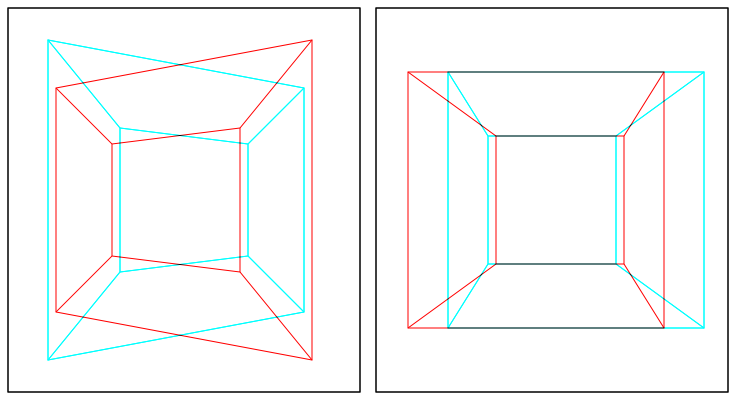
\includegraphics[width=10cm]{pictures/keystoning}
\caption{A 3D cube displayed in toe-in stereo and off-axis stereo (source: \href{http://doc-ok.org/?p=77} {doc-ok.org})}
\label{fig:keystoning}
\end{figure}

Note that this setup is still acceptable for stereo computer vision, which does not really focus about getting acceptable stereopsis and convergence but simply working with as much stereo pairs as possible \cite{book_cv} (how pairs are mapped into depth information is only a matter of calibration). This is also the preferred setup for stereoscopic imaging in photography (where the subject is captured only once and under controlled circumstances) and is still acceptable for video capturing under the assumption that eyes will be most of the time focused on the center of the screen and a good compromise between camera tilt and distance from subject is reached \cite{link_stereo_tricks}.

\subsection{Stereo camera calibration for stereo vision}
Analyzed stereo rig models assume geometric constraints are respected, which is an ideal case. Though human eye can still tolerate slight alignment approximation, stereo computer vision requires precision to obtain reliable data. Stereo calibration process is similar to single camera calibration: it involves more steps, includes getting both intrinsic parameters from each camera and extrinsics for the stereo setup \cite{link_stereo_calib_example}. Camera position and pose are considered in the equation. The aim is to make corresponding epipolar lines in image pairs be parallel to horizontal direction.

We won't analyse all proposed solutions to this problem as this falls beyond the scope of this text. We will however put some effort in considering its relationship with previously mentioned configurations. In order to avoid heavy computation in image undistortion, a recent study \cite{stereo_rectify_parallelise} exploits the relationship between the general-type unconstrained configuration (which is the non-calibrated rig) to its virtual parallel-type equivalent. It is worth mentioning the proposed algorithm avoids completely complex calculations based on epipolar lines or fundamental matrix. The resulting images appear to be considered as if they were captured by a parallel stereo camera rig with its own optical axis sharing the same origin: raw frame points are re-projected into a new plane and after rectification there is no residue of keystoning, at the cost of reducing perceived FOV. However, since original capture is issued by a toed-in configuration, it cannot be considered a real parallel equivalent; only a portion of rectified frame will contain informational content, leaving black areas within view angles reached by the parallel configuration only.

\begin{figure}
\centering
\begin{subfigure}{0.49\textwidth}
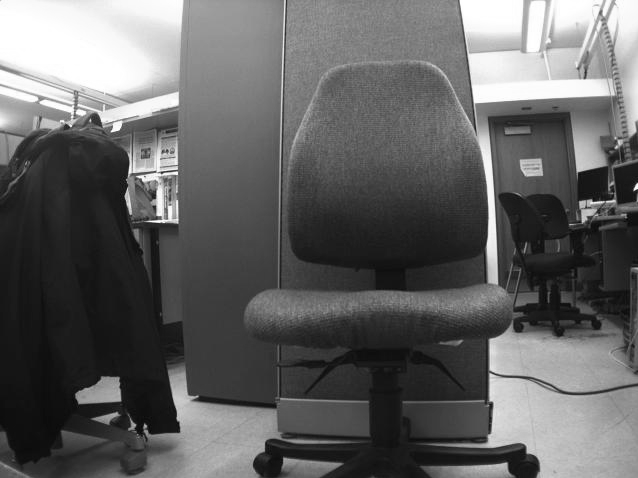
\includegraphics[width=\linewidth, height=5.5cm]{pictures/mono-distorted}
\end{subfigure}
%\hspace{\fill}
\begin{subfigure}{0.49\textwidth}
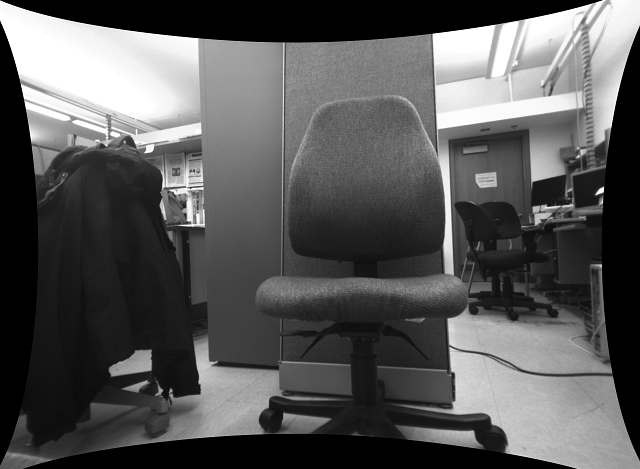
\includegraphics[width=\linewidth, height=5.5cm]{pictures/mono-undistorted}
\end{subfigure}
%\vspace*{2mm}
\caption{Image undistortion on a mono calibrated camera image. The pincushion will be centered in the real main focal point.  (source: \href{http://paulbourke.net/stereographics/stereorender/}{paulbourke.net})}
\label{fig:mono_undistort}
\vspace*{0.4cm}
\begin{subfigure}{0.49\textwidth}
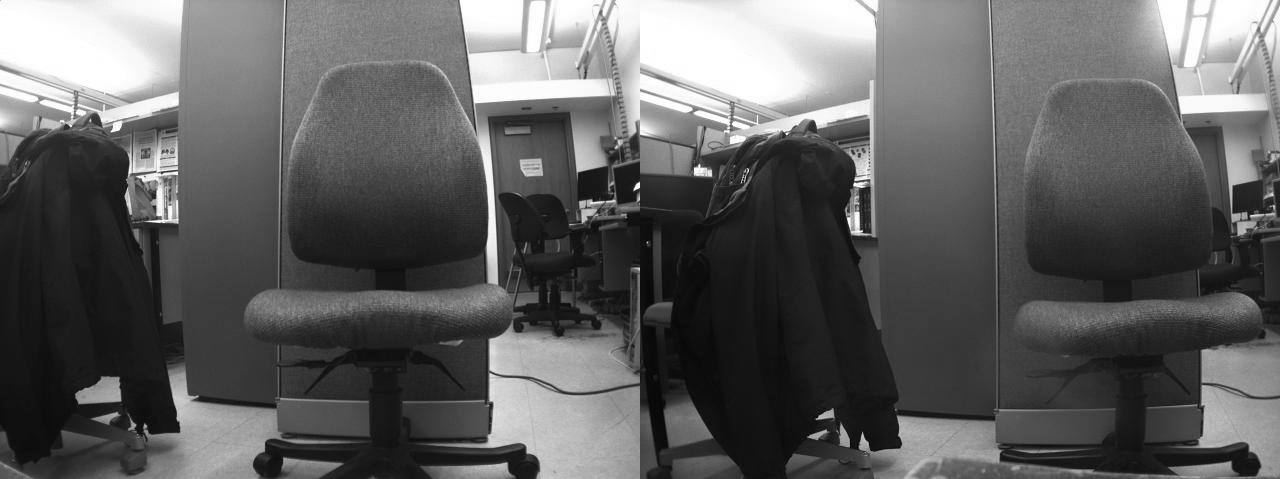
\includegraphics[width=\linewidth]{pictures/stereo-distorted}
\end{subfigure}
\begin{subfigure}{0.49\textwidth}
%\vspace*{0.4cm} % (or whatever vertical separation you prefer)
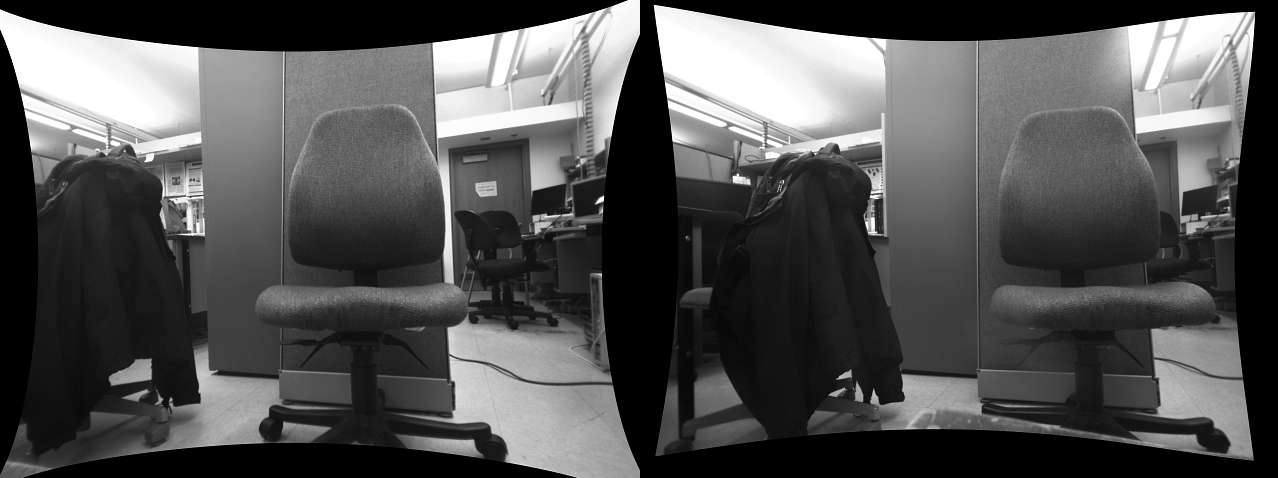
\includegraphics[width=\linewidth]{pictures/stereo-undistorted}
\end{subfigure}
%\vspace*{-6mm}
\caption{Image undistortion on a stereo calibrated camera rig. Note how the two pincushions are also rescaled, rotated or translated relatively so that stereo pairs fall on horizontal lines. (source: \href{http://www.cs.unc.edu/~azuma/ARpresence.pdf}{A Survey of Augmented Reality}). At bottom two respective examples, WorldViz VideoVision powered HMD (left) and Simeye XL100A (right).}
\label{fig:stereo_undistort}
\end{figure}

Stereo calibration is really necessary only where we do not have reasonable control on stereo rig build quality. It is however mandatory for stereo vision algorithms to work properly, which sure is one of the first steps to take to push this work further. Keep in mind that real-time re-sampling of the image is not always feasible and performance is vital to achieve needed FPS. Also consider that effort in getting physical camera alignment right is never too much: FOV is precious and could considerably deteriorate both object detection and user experience \cite{restricting_FOV}.

\subsection{From standard to fish-eye stereo}
A classical tool used in computer vision to capture for acquiring images with large FOV are fish-eye optics. Such lenses can work with a standard CCD or CMOS sensors and remove the need of complex mirror or multiple cameras at the cost of high distortion introduced. The undistortion phase is always necessary even for only displaying image to the user. Since achieving wide FOV falls in our goals, we will also count fish-eye stereo as an option. The challenge to integrate fish-eye projection models into a framework for binocular vision with fish-eye lenses has been previously faced [?], but this regards computer vision only since method is meant to expose the resulting 2D rectified images to automated analysis; in our work we focus also on how to display such images on a non-ordinary display dedicated to immersive applications and how VR, with the results of mono or stereo computer vision, can interact with it.

\section{Modelling first person view in VR}

The stereo oriented approaches presented so far inspired early in the years fields like photography and cinematography, but also later on computer graphics. Virtual reality (VR) is a branch focusing on immersivity, about which we provide an overview of the so called first-person-view (FPV) which aims to reproduce for a user the feel of being (body and mind) in a virtual environment in first person. The reader will agree that FPV modelling is a direct application of what learned so far, under the assumptions . We won't fail to remember  the relevant limitations of simulating a virtual environment and current strategies on how are faced on HMD devices.

\subsection{Head model: IPD and ETN parameters}
Given a 3D virtual environment, stereo in computer graphics can obtained by rendering the same scene from two different view points, much like we do with two cameras in reality. All previously discussed setups can be experimented virtually by implementing custom virtual camera matrices and orienting them in space to achieve desired binocular disparity and convergence. The zero-parallax plane will as well be virtual and can placed in front or behind the real screen. Ideally, how virtual camera should be positioned depends on the display device used and user's distance from it; but over 3D static photography or video footage, a 3D graphics application has a major advantages: applications can assume a initial typical expected case and implement it plus offer options to calibrate the virtual setup, since images are generated at runtime through the virtual cameras. As for user eye convergence, with the support for an eye tracking solution (for example Tobii [?]), it would be possible to adjust virtual orientation dynamically so that correct vergence can be triggered depending on the target object and no precautions must be taken by creator in that sense.

For a video HMD, display is much closer to the eyes and for that to be on focus and to cover human FOV correctly, much more complex optics is involved. Each HMD presents its own implementation of the problem, beginning from user's eye offset up to how virtual camera parameters should be set. Our experiment for instance will be based on a specific HMD set, Oculus Rift Development Kit 2 (DK2), which features wide FOV stereoscopic rendering with suboptimal solution for correct view distortion \cite{link_oculus_limits}. The current work however strives to separate all elements for stereo graphic rendering from the actual display distortion needed.

\begin{figure}
\centering
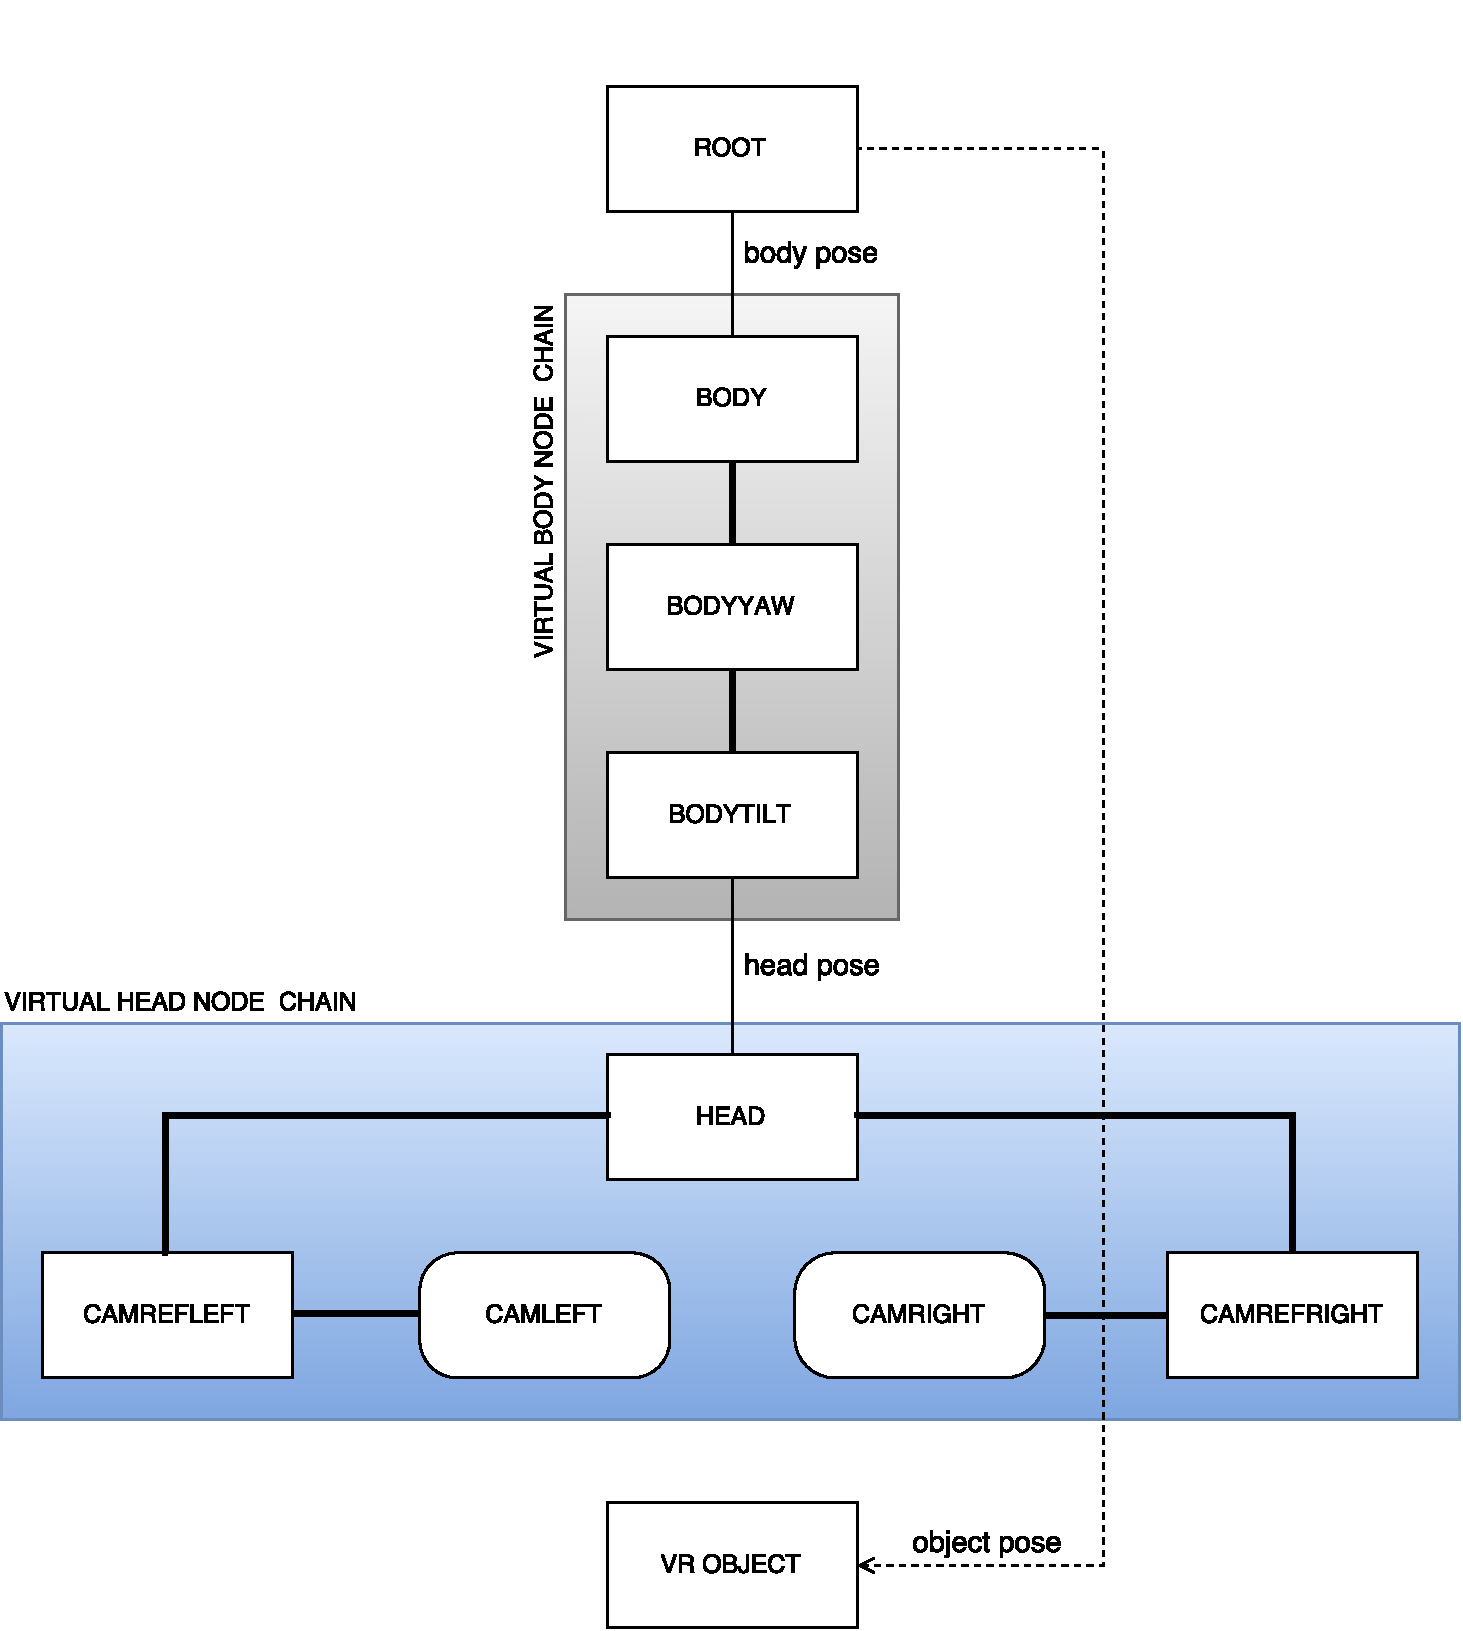
\includegraphics[width=\linewidth]{schemas/classic-head-model_nodetree}
\caption{Thick links indicate nodes with constant position/orientation (for example, IPD and ETN measures) while thinner ones are constantly altered (head pose); body has also been included in the schema for completion, even though body/avatar movements are controlled independently by other means (body tracking or simple controller).}
\label{fig:classic_head_model}
\end{figure}

Given a head-tracked HMD and a stereo graphics application providing a first-person perspective, real and virtual head of the user correspond: each virtual camera will provide point of view for each eye, while their pose in space will be determined by user's head orientation. To get occlusion and parallax cues perfectly coherent to the movements of a real head, virtual inter-camera distance should match real user inter-pupillary distance (IPD): such measure, as also Oculus Rift documentation suggests, must be manually set, together with the actual distance from the eye and neck orbiting point called eye-to-neck distance (ETN). Using a node tree to represent each entity in terms of 3D relative transformation, head model for a first-person perspective VR application appears as in figure N. Camera objects in the schema contain intrinsic parameters defined by HMD requirements: for instance, Oliver Kreylos \cite{link_oculus_limits} confirms Oculus Rift provides specific OpenGL camera parameters to implement off-axis stereo, even though official documentation for the version used of the SDK denies it.

\subsection{Low latency rendering and timewarping}
The schema in figure N displays only how, for a head pose, a 3D scene can be rendered correctly prior to further specific HMD-dependent elaboration of HMD. In practice, the system "sensor-renderer-display" is not instantaneous and each step makes a digital system unto itself, meaning different buffering and filtering phases are involved.

The following work will not focus specifically on head tracking sensors latency issues (dependent from hardware HMD implementation) but will consider more general countermeasures in terms of overall latency, from the time of sensing to video output. On this behalf, the render-display step do require deeper investigation, since recently classic processing model for 3D graphics applications underwent major optimizations for VR in the last couple of years on this matter. Of particular interest and inspiration for this project are "predictive tracking" and "timewarping", which we will briefly describe.

Predictive tracking methods are a very common mitigation technique for reducing latency between a motion sensor capture and its effect on a displayed scene in VR/AR research [?]. Although mathematical methods implied are not recent, they are still very used and improve their performance over time due to improvements in sensing and graphics hardware: recent implementations report very fast and accurate measurements that use low-cost sensors deployed in large variety of virtual reality headsets (from 100 to 30-50ms)\cite{oculus_prediction}. What happens is that, given a delta interval in time that can be fixed or dynamically adjusted, a predicting algorithm assumes a physical cinematic quantity to remain constant over that time in the future and computes from it all derived quantities, such as position and velocity if acceleration is chosen. Error in prediction will obviously increase with longer time intervals, but the time interval itself can be reduced when head motion less fast. By setting time end interval to the estimated time of measure evaluation, latency can be mitigated.

The cited 50ms wall is hard to beat, since render-display latency comes in play, and the ideal "immersive" latency threshold impossible to hit, documented to be 20ms or below \cite{latency_sinequanon}. Even though a sensor measure can be evaluated instantly, the moment it is used in the 3D scene to be rendered, even as a last operation, is still far away from the time of actual display; in other words, there is always a noticeable amount of time between render has started and user sees it.

\begin{figure}
\centering
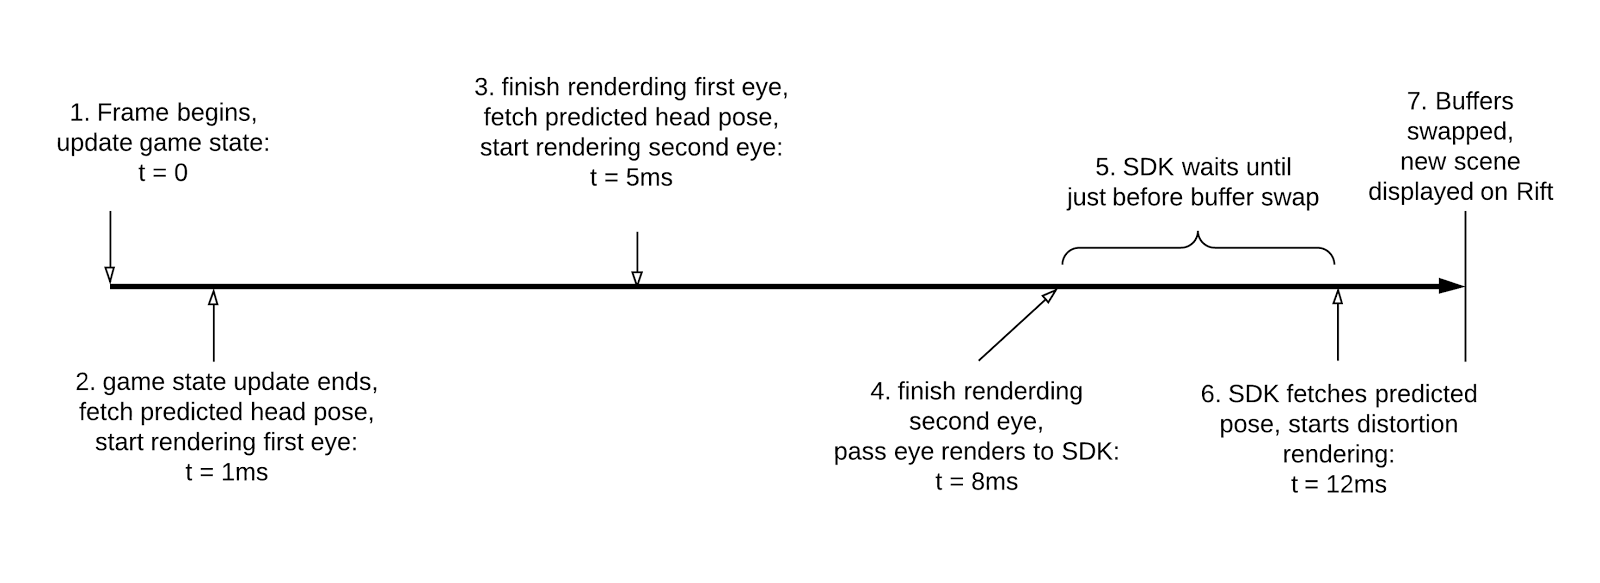
\includegraphics[width=\linewidth]{schemas/timewarp-timeline}
\caption{Render timeline for one frame using pose prediction and asynchronous timewarping. We refer to "SDK" as the part of application that implements those algorithms, not the render pipeline itself. (source: \href{http://rifty-business.blogspot.se/2014/08/using-timewarp-on-oculus-rift.html}{rifty-business.blogspot.se})}
\label{fig:timewarp_timeline}
\end{figure}

According to John Carmack \cite{karmack_mitigation}, moving sensor evaluation up to render phase would have no effect unless hardware is capable to account for that. In its work, he proposes "timewarping" as a state-of-the-art strategy fit for head-tracked HMD to minimize latency perception: by late evaluation of the sensors, one is able to transform and re-project the 2D render result prior to display on screen and fictionally reproduce an movement of the head in the 3D environment. The expected display time (not render) is then fed to the pose prediction algorithm multiple times: the first two measures are set before starting render of each eye and a final third to evaluate the necessary delta transformation to apply each result (schema N). The timewarping transformation cannot produce correct results in terms of occlusion (since it does not correspond to a real rotation of the head model) and also shows its limits at the edges of the render, since culling has already been performed by rendering (example N), but the reported effectiveness in perception is guaranteed by the high frame/refresh rate of the application/HMD, which updates the view before those issues become relevant for user experience.

The implementation of hereby discussed techniques will be taken for granted in our demo application (partial effort is needed with Rift and Oculus SDK) but their results will be discussed and rethought for immersive AR in chapter 3.

\begin{figure} 
\centering   
\begin{subfigure}{0.49\textwidth}
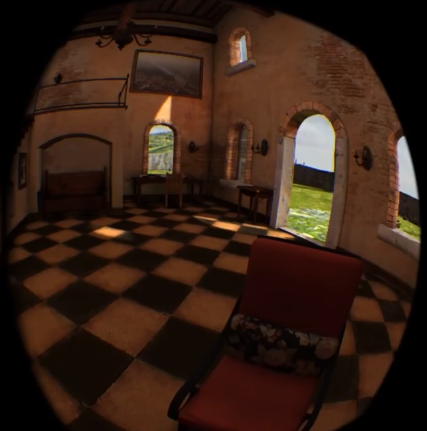
\includegraphics[width=\linewidth, height=7.4cm]{pictures/non-timewarped-chair}
\end{subfigure}
%\hspace{\fill}
\begin{subfigure}{0.49\textwidth}
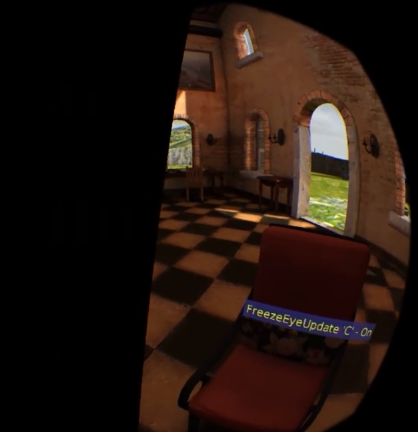
\includegraphics[width=\linewidth, height=7.4cm]{pictures/timewarped-chair}
\end{subfigure}
%\vspace*{2mm}
\caption{The rendered result of a head rotation to the left from the chair at standard FPS (left) and at zero FPS (right). At this extreme conditions, timewarping limits can be appreciated. (source: Oculus "Tuscany" Demo)}
\label{fig:timewarp_example}
\end{figure}

\section{Towards merging real stereo and virtual stereo}

We have seen how to control depth perception with real stereo camera configurations and how it can enhance the simulation of first person view of a virtual scene, which in turn uses virtual model of the real camera. Our next step will be to analyse the relationship between the two and how stereo imagery from virtual and real sources can coexist when both worlds get in contact on a video see-trough HMD device. In the next chapter we will also test the bond and the geometric assumptions made by developing an AR application, while striving to provide feasible solutions to keep the technical and perceptual goals introduced in the first chapter within reach.









\chapter{Proposed solution}



\section{Gear selection}

\subsection{HMD and head tracking}

\subsection{Camera for stereo}
low cost
best resolution/fps rate

\subsection{3D Engine for VR environment}
OculusSDK
Ogre3D

\subsection{Libraries for CV and AR}
OpenCV + tbb + cuda
arUco




\section{Stereo Rig design}

\subsection{wide-angle lens configuration}
TOED-IN
(-) edge violation, "see through a window" effect (lower immersion)
(-) keystoning effect at edges, but reducible
(+) compensate the low stereo cues area of parallel config
(+) easy to implement
(+) good vertical disparities (VSR)

\subsection{fish-eye lens configuration}
PARALLEL with high fov
(+) no edge violation (close objects are welcome, high immersion)
(+) no keystoning
(+) no need to toe-in to compensate low fov..
(-) .. but still can be very distorted at edge (need high quality lens!)
(-) no stereo cues at the edge of the image
(-) hard to implement (due to additional undistortion)
(+) good vertical disparities (VSR)

\subsection{3D printed prototype (?)}


\section{Application pipeline}


\section{Camera image pipeline}

\subsection{Defining capture data}

\subsection{Overcoming }

\subsection{Undistort, feature extraction, image enhancement}

\subsection{Frame synchronization}

\section{Rendering pipeline}

\subsection{Enhanced head model}

\subsection{Distortion handling}

\subsection{3D scene image to eye}

\subsection{Camera image to 3D Scene}

\subsubsection{pin-hole model}
\subsubsection{fish-eye model}



\section{Increasing immersivity}

\subsection{Higher frame rate: decreasing image resolution}

\subsection{Skybox}

\subsection{Fish-eye lenses}

\subsection{Virtual nose}

\subsection{Virtual hands}

\chapter{Experimental results}

We will now present the results of narrow set of experiments aimed to observe both user confort when exposed to different visualization conditions offered by our application (chosen among all the possible setups provided) and to measure performance where the vision pipeline is active.

As a common setting, the 3D rendering engine has been forced to run at 60 fps while each camera runs at its best with 30 fps.  Performance results will be classified by computational hardware used, application setting and camera image resolution.

A consideration must be done for camera resolution. With cameras in stock configuration, the highest 16:9 resolution used in the experiments is 1024x576 (on the 1920x1080 available): the reason is that, since image will not cover the entire HMD FOV with stock wide-angle lenses, it is no use to use the whole sensor surface. Resolution was then further reduced whenever the subject could not perceive any loss in quality (thus improving performance at zero cost) or whenever we needed to experiment with performance to provide more complete results or a reasonable frame rate with hardware in use.\\
The high resolution of the sensor however still comes in handy when dealing with fish-eye lenses: to achieve the highest FOV possible, it is convenient to adjust the lens so that the entire fish-eye circle is restricted into the 16:9 area of the sensor used for video streaming, which in turn explains the need of higher resolution (image will need to be scaled to cover the entire HMD screen).

Machine used for running the demo are:
- Asus U500VZ - i7 3.00 Ghz - Nvidia GT650M (with cuda support)
- "Aragorn" (from cvap) - ...

\section{Live stereo augmented reality demo}
In this experiment we tested the behaviour of the application in wide-angle toed-in configuration, streaming live images from the cameras into the HMD, and presenting them to the user. In addition, the AR pipeline is active and detecting an arUco marker from left camera and placing a virtual object in front of the viewer. To random subjects has been asked to walk around in a room with HMD on and to provide feedback on their experience on 3D perception when watching the marker static or manipulating it. The specific "yes/no" questions posed were:
(questions?)
The experiment was repeated for each subject under four different application settings:
\begin{itemize}
\item dark background and image stabilization off;
\item dark background and image stabilization on;
\item skybox active and image stabilization off;
\item skybox active and image stabilization on.
\end{itemize}
In the following table (N) we have classified the results.

(observations)

\section{CUDA pipeline performance with NPR filter}
In the demo in configuration X from previous paragraph has been activated the image effect pipeline, which uses the camera image and CUDA support to apply a Non-Photorealistic-Reality (NPR) filter. Gooch shading was also used to apply a "toon" effect to the rest of the virtual environment.

The experiment focuses more on performance measurement than user experience, since deeper research and control over virtual environment rendering output is needed to achieve reliable results in terms of psychological perception. We asked anyway a less formal opinion on subjects under test on whether they could still distinguish real objects (from camera image) from the virtual object (from AR pipeline). Tests were performed with both OpenCV undistortion on and off, since we found that undistortion should be implemented in CUDA as well but with our setup arUco was still successfull in detecting the marker properly even without undistortion.

(results)


\section{Offline stereo fish-eye demo}
Since in our experiments we did not have reasonable control over lens replacement and positioning on stock cameras, we proposed an alternative able to test the capabilities of our fish-eye mesh undistortion algorithm implemented in a glsl fragment shader. The experiment shows off static off-line stereo fish-eye imagery so that user can play with different shader settings until image appears undistorted in the view (and covers more than the HMD FOV).

To subjects has been asked (without being able to move but only to rotate their heads around, since image no longer responds to real body movements) how immersed in the scene they felt, even though the scene was only composed of the undistorted fish-eye image.

(results)





\chapter{Conclusions and future work}

\section{Increasing immersivity}

\subsection{Using a Skybox}

\subsection{Employing Fish-eye lenses}
Increased percieved FOV \\
Decouple from camera FPS\\

\subsection{Virtual nose}



\section{Performance optimizations for future applications}

\subsection{Low FPS: decreasing image resolution}

\subsection{Undistort and marker detection in CUDA}

\subsection{"Mono" mode}



\section{Further development}

\subsection{Depth mapping with stereo computer vision}

\subsection{Introducing virtual hands with Leap Motion}

\subsection{Integration with ROS}





\iffalse

Discutere in questo capitolo come � stata progettata la soluzione al problema trattato nella tesi, indicando anche se sono stati valutati vari possibili approcci o soluzioni pre-esistenti e giustificando le proprie scelte. Descrivere quindi la soluzione vera e propria.

Nel caso sia stato sviluppato del software non triviale, � buona norma dedicargli tre sezioni:
\begin{itemize}
\item architettura dell'applicazione (interazioni con gli utenti e con altri sistemi, moduli logici, flussi dati interni ed esterni);
\item manuale dello sviluppatore (descrizione dei moduli, degli algoritmi, delle interfacce e delle strutture dati);
\item manuale utente (come installare ed usare il programma, interfacce, comandi, dati in input ed in output).
\end{itemize}
Nel caso di software molto voluminoso, queste tre sezioni possono diventare tre capitoli separati.

\chapter{Risultati}

Inserire in questo capitolo i risultati conseguiti, cercando di analizzarli -- se possibile -- in modo quantitativo.


\chapter{Conclusioni}

Qui si inseriscono brevi conclusioni sul lavoro svolto, senza ripetere inutilmente il sommario.

Si possono evidenziare i punti di forza e quelli di debolezza, nonch� i possibili sviluppi futuri o attivit� da svolgere per migliorare i risultati.

\fi

% print bibliography
% La bibliografia, da inserirsi solo se ci sono state citazioni.
% In questo caso ricordarsi che bisogna sempre elaborare due volte il file .TEX
% perch� la prima volta viene generata la bibliografia mentre la seconda volta viene inclusa

% NOTA: citare il DOI non � obbligatorio ma MOLTO desiderabile

%\begin{thebibliography}{9} % se ci sono meno di 10 citazioni
\begin{thebibliography}{99} % se ci sono da 10 a 99 citazioni

\bibitem{immersivity_vr}
D. Marini, R. Folgieri, D. Gadia, A. Rizzi,
``Virtual reality as a communication process", Virtual Reality 16, no. 3 (2012): 233-241.


\bibitem{linkzeropoint}
Youtube - ``Zero Point", VR 360 film, \\ \href{https://www.youtube.com/watch?v=DsXEUPS2uss}{https://www.youtube.com/watch?v=DsXEUPS2uss}

\bibitem{link_starwars_trailer}
Facebook - ``Star Wars: The Force Awakens", Immersive 360 Teaser Trailer, \\ \href{https://www.facebook.com/StarWars/videos/1030579940326940/}{https://www.facebook.com/StarWars/videos/1030579940326940/}


\bibitem{immersivity_film}
A. D’Aloia,
``Film in Depth. Water and Immersivity in the Contemporary Film Experience." Acta Universitatis Sapientiae, Film and Media Studies 05 (2012): 87-106.

\bibitem{immersivity_3D}
M. Kozhevnikov, R. P. Dhond,
``Understanding immersivity: image generation and transformation processes in 3D immersive environments." Frontiers in psychology 3 (2012).

\bibitem{book_cv}
R. Hartley and A. Zisserman,
``Multiple View Geometry in Computer Vision", Second Edition, Cambridge University Press, March 2004,
ISBN: 0521540518

\bibitem{ar_intro}
 R. T. Azuma,
``A survey of augmented reality" Presence 6, no. 4 (1997): 355-385.

\bibitem{telepresence_intro}
G. H. Ballantyne,
``Robotic surgery, telerobotic surgery, telepresence, and telementoring", Surgical Endoscopy and Other Interventional Techniques 16, no. 10 (2002): 1389-1402.


\bibitem{vr_presence}
Larry F.~Hodges, Barbara O.~Rothbaum, R.~Kooperα,
D.~Opdyke, T.~Meyer, Johannes J. de Graaff,
James S. Williford, Max M. North,
``Presence as the defining factor in a VR application",
GVU Technical Report, GIT-GVU-94-06,
Georgia Institute of Technology (USA), 1994


\bibitem{link_google_translate_AR}
Google Play App Store - ``Google Translate", formerly World Lens, \\ \href{https://play.google.com/store/apps/details?id=com.google.android.apps.translate}{https://play.google.com/store/apps/details?id=com.google.android.apps.translate}

\bibitem{link_IKEA_AR}
Youtube - ``IKEA AR Catalogue", commercial, \\ \href{https://www.youtube.com/watch?v=vDNzTasuYEw}{https://www.youtube.com/watch?v=vDNzTasuYEw}

\bibitem{milgram_continuum}
P. Milgram, H. Takemura, A. Utsumi, F. Kishino,
``Augmented Reality: A class of displays on the reality-virtuality continuum",
Proc. SPIE 2351, Telemanipulator and Telepresence Technologies, 282 (December 21, 1995), \doi{10.1117/12.197321}

\bibitem{tracking_AR}
R. Azuma,
``Tracking requirements for augmented reality", Communications of the ACM 36, no. 7 (1993): 50-51.




\bibitem{optical_vs_video_st}
J. P. Rolland, H. Fucks,
``Optical Versus Video See-Through Head-Mounted Displays in Medical Visualization",
Massachusetts Institute of Technology, June 2000, Vol. 9, No. 3, Pages 287-309,
\doi{10.1162/105474600566808}

\bibitem{virtual_sickness}
J. J. W. Lin, H. B. Duh, D. E. Parker, H. Abi-Rached, T. Furness,
``Effects of field of view on presence, enjoyment, memory, and simulator sickness in a virtual environment", in Virtual Reality, 2002. Proceedings. IEEE, pp. 164-171. IEEE, 2002.

\bibitem{oculus_rift}
Oculus Rift official homepage, 2015 \\ \href{https://www.oculus.com/en-us/rift/}{www.oculus.com/en-us/rift/}

\bibitem{google_glass}
Google Glass official homepage, 2015 \\ \href{https://www.google.com/glass/start/
}{www.google.com/glass/start/}

\bibitem{microsoft_hololens}
Microsoft Hololens project official homepage, 2015 \\ \href{https://www.microsoft.com/microsoft-hololens/en-us}{www.microsoft.com/microsoft-hololens/en-us}

\bibitem{restricting_FOV}
P. L. Alfano, G. F. Michel
``Restricting the field of view: perceptual and performance effects",
DePaul University, 1990, Perceptual and Motor Skills: Volume 70, Issue , pp. 35-45,
\doi{10.2466/pms.1990.70.1.35}

\bibitem{GPU_accel_stereo_AR}
M. Sizintsev, S. Kuthirummal, S. Samarasekera, R. Kumar, H. S. Sawhney, A. Chaudhry,
``GPU accelerated realtime stereo for augmented reality", 2010, In Proceedings Intl. Symp. 3D Data Processing, Visualization and Transmission (3DPVT)

\bibitem{stereo_rules}
F. Zilly, J. Kluger, P. Kauff,
``Production rules for stereo acquisition", Proceedings of the IEEE 99, no. 4 (2011): 590-606,
\doi{10.1109/JPROC.2010.2095810}

\bibitem{light_field_mapping}
WC. Chen, JY. Bouguet, M. H. Chu, R. Grzeszczuk,
``Light field mapping: efficient representation and hardware rendering of surface light fields", in ACM Transactions on Graphics (TOG), vol. 21, no. 3, pp. 447-456. ACM, 2002.

\bibitem{magic_leap}
Magic Leap project homepage, 2015 \\ \href{http://www.magicleap.com/}{magicleap.com}

\bibitem{disparity_depth}
N. Quian,
``Binocular Disparity and the Perception of Depth",
Neuron, Elsevier, Volume 18, Issue 3, p359–368, March 1997,
\doi{10.1016/S0896-6273(00)81238-6}



\bibitem{stereoscopic_3D_acquisition}
M. Hasmanda, K. Riha,
``The Modelling of Stereoscopic 3D Scene Acquisition",
Brno University of Technology, April 2012, cited from paragraph 1.1

\bibitem{correct_stereo_pairs}
P. Burke,
``Creating correct stereo pairs from any raytracer",
SPIE Three Dimensional Imaging and Remote Sensing Imaging, Vol 902, pp 85, 2001

\bibitem{camera_convergence}
R. S. Allison,
``The Camera Convergence Problem Revisited",
Department of Computer Science and Centre for Vision Research, York
University, 2004,
\doi{10.1.1.145.9490}

\bibitem{dynamic_virtual_eye_convergence}
A. Sherstyuk, A. Dey, C. Sandor,
``Dynamic eye convergence for head-mounted displays improves user performance in virtual environments",
Proceedings of the ACM SIGGRAPH Symposium on Interactive 3D Graphics and Games. ACM, 2012


\bibitem{offaxis_frustrums}
P. Burke,
``Offaxis frustums: What are they and what are they good for?"
Centre For Astrophysics and Supercomputing, Swinburne University, HET409, September 2004

\bibitem{link_toein_diffused}
O. Kreylos,
``Good Stereo vs Bad Stereo", a brief story of most diffused stereo technique, 2012 \\ \href{http://doc-ok.org/?tag=lens-shift}{http://doc-ok.org/?tag=lens-shift}

\bibitem{link_arrift}
W. Steptoe,
``AR-Rift", Augmented reality project for NPR perception, 2014 \\ \href{http://willsteptoe.com/post/66968953089/ar-rift-part-1}{http://willsteptoe.com/post/66968953089/ar-rift-part-1}

\bibitem{link_stereo_tricks}
D. E. Simanek,
``Digital stereo photography tricks and effects" \\ \href{https://www.lhup.edu/~dsimanek/3d/stereo/tricks.htm}{https://www.lhup.edu/~dsimanek/3d/stereo/tricks.htm}
May, 2010

\bibitem{link_stereo_calib_example}
J. Rambhia,
``Stereo Calibration", an example of stereo calibration using OpenCV \\ \href{http://www.jayrambhia.com/blog/stereo-calibration/}{http://www.jayrambhia.com/blog/stereo-calibration/}
March, 2013

\bibitem{stereo_rectify_parallelise}
H. Su, B. W. He,
``Stereo rectification of calibrated image pairs based on geometric transformation",
I.J. Modern Education and Computer Science (MECS), 2011, 4, 17-24

\bibitem{link_oculus_limits}
O. Kreylos
``A Closer Look at the Oculus Rift", March 2014, \\ \href{http://doc-ok.org/?p=756}{http://doc-ok.org/?p=756}

\bibitem{oculus_prediction}
LaValle, Steven M., Anna Yershova, Max Katsev, and Michael Antonov. ``Head tracking for the Oculus Rift." In Robotics and Automation (ICRA), 2014 IEEE International Conference on, pp. 187-194. IEEE, 2014.

\bibitem{latency_sinequanon}
M. Abrash,
``Latency: the sine qua non of AR and VR", December 2012 \\ \href{http://blogs.valvesoftware.com/abrash/latency-the-sine-qua-non-of-ar-and-vr}{http://blogs.valvesoftware.com/abrash/latency-the-sine-qua-non-of-ar-and-vr}

\bibitem{karmack_mitigation}
J. Carmack, ``Latency mitigation strategies", Feb. 2013 \\ Backup link: \href{https://www.twentymilliseconds.com/post/latency-mitigation-strategies/}{https://www.twentymilliseconds.com/post/latency-mitigation-strategies/}






\bibitem{stereo_pair_cameras}
P. Burke,
``Calculating Stereo Pairs", 1999 \\ \href{http://paulbourke.net/stereographics/stereorender/}{http://paulbourke.net/stereographics/stereorender/}

\bibitem{keystone_correction}
R. Sukthankar, R. Stockton, M. Mullin,
``Automatic Keystone Correction for Camera-assisted Presentation Interfaces",
Proceedings of International Conference on Multimedia Interfaces,
October, 2000

\bibitem{stereo_pairs_game}
P. Burke,
``Create side-by-side stereo pairs in the Unity game engine", 2008 \\ \href{http://paulbourke.net/stereographics/Unitystereo/}{http://paulbourke.net/stereographics/Unitystereo/}


\bibitem{sub2r}
SUB2R - High speed cameras for computer vision \\ \href{http://www.sub2r.com}{http://www.sub2r.com}

\bibitem{ptgrey}
PTGREY - High speed cameras for computer vision \\ \href{http://www.ptgrey.com}{http://www.ptgrey.com}

\bibitem{ar_rift}
W. Steptoe, S. Julier, A. Steed,
``Presence and Discernability in Conventional and Non-Photorealistic Immersive Augmented Reality",
Mixed and Augmented Reality (ISMAR), 2014 IEEE International Symposium on. IEEE, 2015,
\doi{10.1109/ISMAR.2014.6948430}




\bibitem{fisheye_lens}
D. Brooks,
`` Lenses and lens accessories: a photographer's guide", 1982, p. 29. \\ISBN: 9780930764340.

\bibitem{book_stereographic_projection}
R. J. Lisle, P. R. Leyshon,
``Stereographic Projection Techniques for Geologists and Civil Engineers",
Cambridge University Press, 2004
\doi{10.1017/CBO9781139171366}

\bibitem{immersive_displays}
E. Lantz, 
``A survey of large-scale immersive displays", Proceedings of the 2007 workshop on Emerging displays technologies: images and beyond: the future of displays and interaction, ACM International Conference Proceeding Series; Vol. 252, 2007,
\doi{10.1145/1278240.1278241}

\bibitem{omni_fisheye}
P. Burke,
``Omni-directional Stereoscopic Fisheye Images for Immersive Hemispherical Dome Environments",
WASP, University of Western Australia, Computer Games and Allied Technology,136-143, 2009

\bibitem{cg_projections}
D. Salamon, 
``Transformations and Projections in Computer Graphics", Springer London, pp 145-220, 2005,
\doi{10.1007/978-1-84628-620-9}


\bibitem{link_dissecting_camera_matrix}
K. Simek, ``Dissecting the camera matrix", June 2013\\ \href{http://ksimek.github.io/2013/06/03/calibrated\_cameras\_in\_opengl/}{http://ksimek.github.io/2013/06/03/calibrated\_cameras\_in\_opengl/}


\bibitem{cg_rendering}
N. Kurachi, 
``The magic of computer graphics", CRC Press, cited from Chapter 5: "image based rendering", 2011,\\
Print ISBN: 978-1-56881-577-0\\
eBook ISBN: 978-1-4398-7357-1

\bibitem{link_vrui}
VRUI - Vrui Toolkit Official Homepage \\ \href{http://idav.ucdavis.edu/~okreylos/ResDev/Vrui/}{http://idav.ucdavis.edu/~okreylos/ResDev/Vrui/}

\bibitem{link_fisheye_undistortion}
Stackoverflow - ``Correcting Fisheye Distortion Programmatically", an example result of fish-eye undistortion and its problems \\ \href{http://stackoverflow.com/questions/2477774/correcting-fisheye-distortion-programmatically}{http://stackoverflow.com/questions/2477774/correcting-fisheye-distortion-programmatically}

\bibitem{precise_fisheye_calib}
M. Kedzierski, P. Walczykowski, R. Kaczynski,
``Precise calibration of fisheye lens camera system and projection model", 2006

\bibitem{link_calib3d_opencv}
OpenCV - Calib3d implementation in OpenCV for fisheye model \\ \href{http://docs.opencv.org/master/db/d58/group_\_calib3d_\_fisheye.html}{http://docs.opencv.org/master/db/d58/group\_\_calib3d\_\_fisheye.html}


\bibitem{link_matlab_ocamcalib}
OcamCalib - Camera calibration tool for Matlab \\ \href{https://sites.google.com/site/scarabotix/ocamcalib-toolbox}{https://sites.google.com/site/scarabotix/ocamcalib-toolbox}

\bibitem{link_aruco_ogre}
arUco - Example with Ogre3D \\ \href{https://www.youtube.com/watch?v=CzD48UkGsK8}{https://www.youtube.com/watch?v=CzD48UkGsK8}

\bibitem{link_optimized_undistort_opencv}
openCV - How to improve OpenCV performance on lens undistortion from a video feed \\ \href{http://blog.nishihara.me/opencv/2015/09/03/how-to-improve-opencv-performance-on-lens-undistortion-from-a-video-feed/}{http://blog.nishihara.me/opencv/2015/09/03/how-to-improve-opencv-performance-on-lens-undistortion-from-a-video-feed/}

\bibitem{leap_motion}
Leap Motion official homepage, 2015 \\ \href{https://www.leapmotion.com/}{www.leapmotion.com}

\iffalse
\fi


\end{thebibliography}



\end{document}
